\documentclass[10pt,a4paper]{report}
% \documentclass[10pt,a4paper]{book} % Uncomment this for print

% ----------------------------------------------------------------------
%  Preamble
% ----------------------------------------------------------------------
% There is some important stuff in the preamble. Go check it out!
% ----------------------------------------------------------------------
% General info
% ----------------------------------------------------------------------
\newcommand{\thesisTitle}{The title of a renowned thesis in the field}
\newcommand{\thesisSubtitle}{Very renowned} % Go to cover.tex file for a subtitle on the cover page
\newcommand{\thesisAuthor}{Chanandler Bong}
\newcommand{\thesisCourse}{Electrical and Computer Engineering}
\newcommand{\thesisSupervisor}{Prof. Full Name}
\newcommand{\thesisChairperson}{Prof. Full Name}
\newcommand{\thesisCommiteeMember}{Prof. Full Name}
\newcommand{\thesisKeywords}{template, msc, tecnico, thesis}
\newcommand{\thesisPalavraasChave}{template, mestrado, tecnico, tese}
\newcommand{\thesisDate}{October 2022}

% ----------------------------------------------------------------------
% Fonts
% ----------------------------------------------------------------------
\renewcommand{\rmdefault}{phv} % Roman (i.e. serified) font family
\renewcommand{\sfdefault}{phv} % Sans serif font family
\renewcommand{\ttdefault}{lmtt} % Monospaced (i.e. typewritter-like) font family

\def\FontLn{% 16 pt normal
    \usefont{T1}{phv}{m}{n}\fontsize{16pt}{16pt}\selectfont}
\def\FontLb{% 16 pt bold
    \usefont{T1}{phv}{b}{n}\fontsize{16pt}{16pt}\selectfont}
\def\FontMn{% 14 pt normal
    \usefont{T1}{phv}{m}{n}\fontsize{14pt}{14pt}\selectfont}
\def\FontMb{% 14 pt bold
    \usefont{T1}{phv}{b}{n}\fontsize{14pt}{14pt}\selectfont}
\def\FontSn{% 12 pt normal
    \usefont{T1}{phv}{m}{n}\fontsize{12pt}{12pt}\selectfont}

% ----------------------------------------------------------------------
% Page layout
% ----------------------------------------------------------------------
% Page margins
\usepackage{geometry}
\geometry{verbose,tmargin=2.5cm,bmargin=2.5cm,lmargin=2.5cm,rmargin=2.5cm}

% Line spacing
\usepackage{setspace}
\renewcommand{\baselinestretch}{1.5}
% \doublespacing

% Indent before all paragraphs
\usepackage{indentfirst}

% ----------------------------------------------------------------------
% Hyperlinks
% ----------------------------------------------------------------------
\usepackage[pdftex]{hyperref} % enhance documents that are to be output as HTML and PDF
\hypersetup{colorlinks, % Eliminates borders around links
    linkcolor=black, % Color for normal internal links
    anchorcolor=black, % Color for anchor text
    citecolor=black, % Color for bibliographical citations
    filecolor=black, % Color for URLs which open local files
    menucolor=black, % Color for Acrobat menu items
    urlcolor=cyan, % Color for linked URLs
    bookmarksopen=false, % Don't expand bookmarks
    bookmarksnumbered=true, % Number bookmarks
    pdftitle={\thesisTitle},
    pdfauthor={\thesisAuthor},
    pdfsubject={\thesisCourse},
    pdfkeywords={\thesisKeywords},
    pdfstartview=FitV,
    pdfdisplaydoctitle=true}

\usepackage[acronym,nonumberlist]{glossaries} % Must be loaded after hyperref. Option acronym is for separate list of  acronyms. Option nonumberlist is for not listing the pages in which an entry has been indexed.
\newglossary{nomenclature}{nmc}{nml}{Nomenclature}
\makeglossaries

\usepackage[numbers,sort&compress]{natbib}
\bibliographystyle{IEEEtranN} % Change here the bibliography style for your document

\usepackage{notoccite}

% ----------------------------------------------------------------------
% Graphics
% ----------------------------------------------------------------------
% Color support
\usepackage[table, dvipsnames]{xcolor} % Table option loads  the colortbl package (allows coloring rows, columns, and cells within tables).

% Image support
\usepackage{graphicx}
\usepackage{wrapfig} % Tro wrap text around figure.

% Captions
\usepackage[font=footnotesize,labelfont=bf]{caption}
\usepackage{subcaption}

% Landscape support for images and tables
\usepackage{rotating} % Use \begin{sidewaystable} and \begin{sidewaysfigure}

% Table support
\usepackage{dcolumn} % Alignment of tabular columns
\newcolumntype{d}{D{.}{.}{-1}} % column aligned by the point separator '.'
\newcolumntype{e}{D{E}{E}{-1}} % column aligned by the exponent 'E'
\usepackage{multirow}
\usepackage{booktabs}

% For colored boxes
\usepackage{tcolorbox}

% ----------------------------------------------------------------------
% Technical
% ----------------------------------------------------------------------
% Math
\usepackage{amsmath}
\usepackage{amsthm}
\usepackage{amsfonts}

% Programming
\usepackage{algorithm}
\usepackage{algpseudocode}

% ----------------------------------------------------------------------
% Language
% ----------------------------------------------------------------------
% Encoding
\usepackage[utf8]{inputenc}

% Language
\usepackage[english]{babel}
\selectlanguage{english}

\newcommand{\acknowledgments}{@undefined}
\newcommand{\abstractnamept}{@undefined}
\newcommand{\nomname}{@undefined}

\addto\captionsenglish{\renewcommand{\abstractname}{Abstract}}
\addto\captionsenglish{\renewcommand{\abstractnamept}{Resumo}}
\addto\captionsenglish{\renewcommand{\acknowledgments}{Acknowledgments}}
\addto\captionsenglish{\renewcommand{\contentsname}{Contents}}
\addto\captionsenglish{\renewcommand{\listtablename}{List of Tables}}
\addto\captionsenglish{\renewcommand{\listfigurename}{List of Figures}}
\addto\captionsenglish{\renewcommand{\glossaryname}{Glossary}}
\addto\captionsenglish{\renewcommand{\acronymname}{Acronyms}}
\addto\captionsenglish{\renewcommand{\nomname}{Nomenclature}}
\addto\captionsenglish{\renewcommand{\bibname}{References}}
\addto\captionsenglish{\renewcommand{\appendixname}{Appendix}}

% ----------------------------------------------------------------------
% Additional features
% ----------------------------------------------------------------------
% Underlining
\usepackage[normalem]{ulem}

% Dates with consistent layouts
\usepackage[en-US]{datetime2}

% Customize enumerate labels
\usepackage[inline,shortlabels]{enumitem}

% For \tab command
\usepackage{tabto}

% For "horizontal lists"
\usepackage{multicol} % Same as enumitem inline

% For stylish quotes
\usepackage{csquotes}

% For code
\usepackage{listings}
\definecolor{codegreen}{rgb}{0,0.6,0}
\definecolor{codegray}{rgb}{0.5,0.5,0.5}
\definecolor{codepurple}{rgb}{0.58,0,0.82}
\definecolor{backcolour}{rgb}{0.95,0.95,0.92}
\lstdefinestyle{mystyle}{
    backgroundcolor=\color{backcolour},
    commentstyle=\color{codegreen},
    keywordstyle=\color{magenta},
    numberstyle=\tiny\color{codegray},
    stringstyle=\color{codepurple},
    basicstyle=\ttfamily\footnotesize,
    breakatwhitespace=false,
    breaklines=true,
    captionpos=b,
    keepspaces=true,
    numbers=left,
    numbersep=5pt,
    showspaces=false,
    showstringspaces=false,
    showtabs=false,
    tabsize=2
}
\lstset{style=mystyle}

% For directory trees
\usepackage{dirtree}
\renewcommand*\DTstylecomment{\sffamily\footnotesize\selectfont}

\usepackage{pdfpages}

% ----------------------------------------------------------------------
% Commands
% ----------------------------------------------------------------------
\newcommand{\coverThesis}{Thesis to obtain the Master of Science Degree in}
\newcommand{\coverSupervisors}{Supervisor}
\newcommand{\coverExaminationCommittee}{Examination Committee}
\newcommand{\coverChairperson}{Chairperson}
\newcommand{\coverSupervisor}{Supervisor}
\newcommand{\coverMemberCommittee}{Member of the Committee}

% For degree symbol
\renewcommand{\deg}{$^\circ \ $}

% For feature box (uses tcolorbox package)
\newtcolorbox[]{feature}[1]{
    title={\textbf{Feature} #1},
}



\begin{document}

% Input acronyms and glossary before any text
\newglossaryentry{roll}
{
	type=nomenclature,
	name={$\phi$},
	description={Roll}
}

\newglossaryentry{pitch}
{
	type=nomenclature,
	name={$\theta$},
	description={Pitch}
}

\newglossaryentry{yaw}
{
	type=nomenclature,
	name={$\psi$},
	description={Yaw}
}
\newacronym{ist}{IST}{Instituto Superior Técnico}

\newacronym{monarch}{MOnarCH}{Multi-Robot Cognitive Systems Operating in Hospitals}
\newglossaryentry{mentioned_definition}
{
  name={mentioned definition},
  description={A mentioned definition is a definition that is mentioned throughout the length of the text and is therefore shown in the glossary.}
}

\newglossaryentry{unmentioned_definition}
{
  name={unmentioned definition},
  description={An unmentioned definition is a definition that is not mentioned throughout the length of the text and is therefore will not be listed in the glossary.}
}

% ----------------------------------------------------------------------
%  Cover
% ----------------------------------------------------------------------
\pagestyle{plain} % No headers, footer with centered page number
\pagenumbering{roman} % Set roman numbering (i,ii,...)
\thispagestyle {empty}

% IST Logo - Signature A
% parameters: bb=llx lly urx ury (bounding box), width=h_length, height=v_length, angle=angle, scale=factor, clip=true/false, draft=true/false. 

\includegraphics[bb=9.5cm 11cm 0cm 0cm,scale=0.29]{images/ist_logo.pdf}

\begin{center}
    %
    % Figure (Image or plot)
    \vspace{2.5cm}
    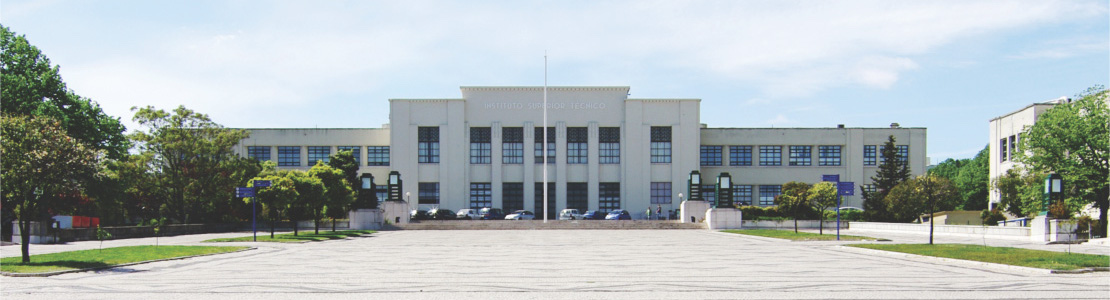
\includegraphics[height=40mm]{images/ist_alameda_1.jpg}

    % Title, author and degree
    \vspace{1.0cm}
    {\FontLb \thesisTitle} \\
    %%%%%%%%%%%%%%%% COMMENT THIS FOR NO SUBTITLE %%%%%%%%%%%%%%%%
    \vspace{0.5cm}
    {\FontMn \thesisSubtitle} \\
    \vspace{1.2cm}
    %%%%%%%%%%%%%%%%%%%%%% AND COMMENT THIS %%%%%%%%%%%%%%%%%%%%%%
    % \vspace{2.6cm}
    %%%%%%%%%%%%%%%%%%%%%%%%%%%%%%%%%%%%%%%%%%%%%%%%%%%%%%%%%%%%%%
    {\FontMb \thesisAuthor} \\
    \vspace{1.2cm}
    {\FontSn \coverThesis} \\
    \vspace{0.3cm}
    {\FontLb \thesisCourse} \\
    \vspace{1.0cm}
    {\FontSn %
        \begin{tabular}{ll}
            \coverSupervisors: \thesisSupervisor
        \end{tabular} } \\
    \vspace{1.0cm}
    {\FontMb \coverExaminationCommittee} \\
    \vspace{0.3cm}
    {\FontSn %
        \begin{tabular}{c}
            \coverChairperson:     \thesisChairperson \\
            \coverSupervisor:      \thesisSupervisor  \\
            \coverMemberCommittee: \thesisCommiteeMember
        \end{tabular} } \\
    \vspace{1.5cm}
    {\FontMb \thesisDate} \\
\end{center}

\newpage

% ----------------------------------------------------------------------
%  Abstract
% ----------------------------------------------------------------------
\section*{\abstractname}

Insert your abstract here.

\vfill

\textbf{\Large Keywords:} \thesisKeywords.


\addcontentsline{toc}{section}{\abstractname}

\pagebreak

\section*{\abstractnamept}

O ``abstract'' em português vai aqui!

\vfill

\textbf{\Large Palavras-chave:} \thesisPalavraasChave.
\addcontentsline{toc}{section}{\abstractnamept}

% ----------------------------------------------------------------------
%  Table of contents
% ----------------------------------------------------------------------
\tableofcontents
\addtocontents{toc}{\protect{\pdfbookmark[1]{\contentsname}{toc}}} % Show toc as a pdf bookmark but don't list it in the toc itself

\phantomsection
\addcontentsline{toc}{section}{\listfigurename}
\listoffigures

\phantomsection
\addcontentsline{toc}{section}{\listtablename}
\listoftables

\phantomsection
\addcontentsline{toc}{section}{\glossaryname}
\printglossary

\phantomsection
\addcontentsline{toc}{section}{\acronymname}
\printglossary[type=\acronymtype]

\phantomsection
\addcontentsline{toc}{section}{\nomname}
\printglossary[type=nomenclature,style=tree]


\setcounter{page}{1}
\pagenumbering{arabic}

% ----------------------------------------------------------------------
%  Chapters
% ----------------------------------------------------------------------
\chapter{Introduction}
\label{chapter:introduction}

\section{About the template}

This Master's thesis template isn't just a pretty face! It also comes with a set of examples on:

\begin{itemize}
    \item How to use glossary definitions, acronyms and nomenclature;
    \item How to include images in different layouts (either using the subimage or the minipage methods);
    \item How to cite from the bibliography (.bib) file;
    \item How to insert pretty contrast boxes for relevant notes;
    \item How insert a formatted piece of code;
    \item How insert a directory tree.
\end{itemize}

Don't forget to read de README.md file with more important information such as:

\begin{itemize}
    \item How to build your final pdf document;
    \item How to set up VSCode, the superior IDE (sorry Vim lovers), as local ``Overleaf'';
\end{itemize}

This template follows the guide provided by Técnico on how a Master's thesis should be formatted as per 2022. You can find the guide and a whole lot of gusty info on how to write your thesis \href{https://tecnico.ulisboa.pt/en/education/study-at-tecnico/academic-information/masters-dissertation/}{here}.

\section{Credit where credit is due}

This pretty template is an adapted and more recent version of Prof. André Marta's template. You can find the original template along with an extended abstract template \href{https://fenix.tecnico.ulisboa.pt/homepage/ist31052/documentos-para-elaboracao-da-tese}{here}.

The images I am using are not mine. Here is a list of their authors and URLs:

\begin{itemize}
    \item The Técnico Alameda campus photo on the cover was taken from Técnico's website: \url{https://tecnico.ulisboa.pt/files/2015/07/campus-alameda-banner21.jpg};
    \item The ISTSat-1 image is from the ``110 Histórias, 110 Objetos'' podcast for the ISTSat-1 episode: \url{https://tecnico.ulisboa.pt/files/2022/02/110-historias-110-objetos-o-istsat-1.jpg};
    \item The robot in the appendix is Gasparzinho which was designed as part of the \acrshort{monarch} project. The image was taken from Técnico's website: \url{https://tecnico.ulisboa.pt/files/2015/10/monarch.jpg}.
\end{itemize}




\chapter{Literature Review}
\label{chapter:literature_review}

\section{How to use the glossary, acronyms and nomenclature}

The glossary, acronym and nomenclature entries must all be listed in the ``glossary.tex'', ``acronym.tex'' and ``nomenclature.tex'' files, respectively. 

If you want to mention a term that is defined in your glossary, do this: \gls{mentioned_definition}. If you check the ``glossary.tex'' file, you will see that there is one more definition there which isn't printed out in the pdf document. This is because glossary entries that are not invoked throughout the text are not printed out to the final document. \textbf{This is also true for acronyms, nomenclature and bibliography entries}.

If you want to use an acronym you can do it in many ways, such as:
\begin{itemize}
	\item This: \acrshort{ist};
	\item This: \acrlong{ist};
	\item And this: \acrfull{ist};
	\item The glossaries package can also be used for a nomenclature list. You call the listed nomenclature like you would a regular glossary entry, like this: \gls{roll}, \gls{pitch} and \gls{yaw}.
\end{itemize} 


\section{How to cite from your bibliography file}

If you don't know what a bibliography file looks like, go check out the contents of this document's bib file: ``references.bib''. If your bibliography is small and you can afford to create a bib file by hand, go ahead. However, if your bibliography is too big and/or you'd like to learn how to automatically add entries to your bib file without having to copy and paste stuff from the browser, check out the README.md file!

After a bibliography entry has been added to your bib file you can now cite it. Here are several ways to cite:

\begin{itemize}
	\item You can cite normally like this: \cite{reynaud22_iberspeech};
	\item What if you also want to include the author's name? Do this: \citet{reynaud22_iberspeech};
	\item For just the author's name: \citeauthor{reynaud22_iberspeech};
\end{itemize} 

\begin{tcolorbox}[title=A note on citations]
	As you probably know there are several citation styles. This document is using the IEEE citation style. If you wish to change the citation style loo for the natbib package within the ``preamble.tex'' file and change the ``IEEEtranN'' part to your desired bibliography style.
\end{tcolorbox}




\chapter{Developed work}
\label{chapter:developed_work}

\section{How to add formatted code}

In the developed work section you will probably want to add some code you developed. You can use the listings package to do this. 

\begin{lstlisting}[language=Python]
import numpy as np
	
def incmatrix(genl1,genl2):
	m = len(genl1)
	n = len(genl2)
	M = None #to become the incidence matrix
	VT = np.zeros((n*m,1), int)  #dummy variable
	
	#compute the bitwise xor matrix
	M1 = bitxormatrix(genl1)
	M2 = np.triu(bitxormatrix(genl2),1) 

	for i in range(m-1):
		for j in range(i+1, m):
			[r,c] = np.where(M2 == M1[i,j])
			for k in range(len(r)):
				VT[(i)*n + r[k]] = 1;
				VT[(i)*n + c[k]] = 1;
				VT[(j)*n + r[k]] = 1;
				VT[(j)*n + c[k]] = 1;
				
				if M is None:
					M = np.copy(VT)
				else:
					M = np.concatenate((M, VT), 1)
				
				VT = np.zeros((n*m,1), int)
	
	return M
\end{lstlisting}

This example was taken from the Overleaf documentation, \href{https://www.overleaf.com/learn/latex/Code_listing}{here}.

\section{How to add a directory trees}

Check this project's directory tree in Figure \ref{fig:directory_structure} for more information on each file.

\begin{figure}[!htb]
    \dirtree{%
    .1 /.
	.2 .vscode\DTcomment{VSCode settings. Delete it if you're not using VSCode}.
	.3 \dots.
    .2 images\DTcomment{Store your images here}.
	.3 \dots.
	.2 .gitignore\DTcomment{Some files shouldn't be saved to the repo. Here is a template .gitignore file}.
	.2 .latexmkrc\DTcomment{RC file for latexmk. If you're using Overleaf you don't need this.}.
    .2 abstract.tex.
	.2 acronyms.tex\DTcomment{Acronym entries go here}.
	.2 appendices.tex.
	.2 conclusion.tex.
	.2 cover.tex\DTcomment{Document cover page}.
	.2 developed\_work.tex.
	.2 glossary.tex\DTcomment{Glossary entries go here}.
	.2 introduction.tex.
	.2 literature\_review.tex.
	.2 Makefile\DTcomment{Project's makefile needed to compile project to pdf}.
	.2 nomenclature.tex\DTcomment{Nomenclature entries go here}.
	.2 preamble.tex\DTcomment{File with all needed packages and custom commands}.
	.2 references.bib\DTcomment{Bibliography file}.
	.2 results.tex.
	.2 resumo.tex\DTcomment{Abstract in Portuguese}.
	.2 thesis.pdf\DTcomment{Output pdf file}.
	.2 thesis.synctex.gz\DTcomment{Synctex file needed to navigate directly from code to pdf and vice-versa}.
	.2 thesis.tex\DTcomment{Project's main file which calls all other files}.
    }

    \caption{This project's directory structure.}
    \label{fig:directory_structure}
\end{figure}

\section{How to add tables}

You can create a table using \LaTeX. Use \href{https://www.tablesgenerator.com/}{this} \LaTeX table generator to help you out.

\begin{table}[!htb]
	\centering
	\caption{A simple table with dummy values.}
	\begin{tabular}{|l|l|l|}
		\hline
			  & column 1 & column 2 \\ \hline
		row 1 & 1        & 2        \\ \hline
		row 2 & 3        & 4        \\ \hline
	\end{tabular}
	\label{tab:simple_table}
\end{table}

You can also include tables which are images instead of tabulars. To do this, create your own table, screenshot it and include it in your document as a table (as opposed to a figure). Like this:

\begin{table}[!htb]
	\centering
	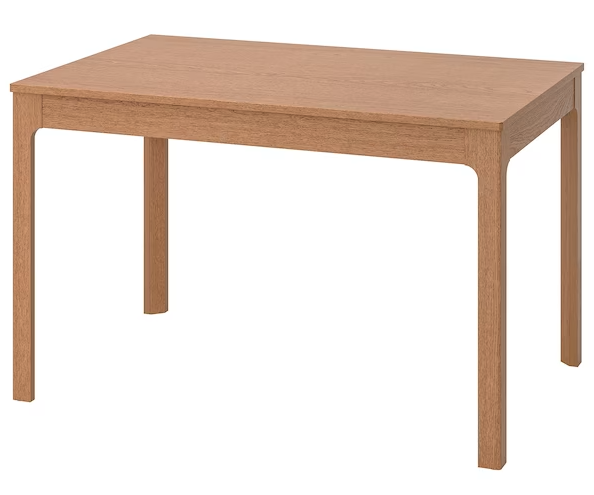
\includegraphics[width=0.5\textwidth]{images/table.png}
	\caption{Another simple table. As you can see anything can be a table in \LaTeX! Don't lose too much time trying to create all your tables using the tabular environment.}
	\label{tab:table_table}
\end{table}

\begin{tcolorbox}[title=A note on table captions]
	Most people prefer table captions to show above the table itself. However, since the guide provided by Técnico (which you can find \href{https://tecnico.ulisboa.pt/en/education/study-at-tecnico/academic-information/masters-dissertation/}{here}) doesn't specify a specific placement, this is a matter of opinion. If you want your table caption to be above the table use the example of Table \ref{tab:simple_table}, otherwise use the example of Table \ref{tab:table_table}.
\end{tcolorbox}


\chapter{Results}
\label{chapter:results}

\section{How to add images}

A simple image can be added like this.

\begin{figure}[!htb]
	\centering
	
	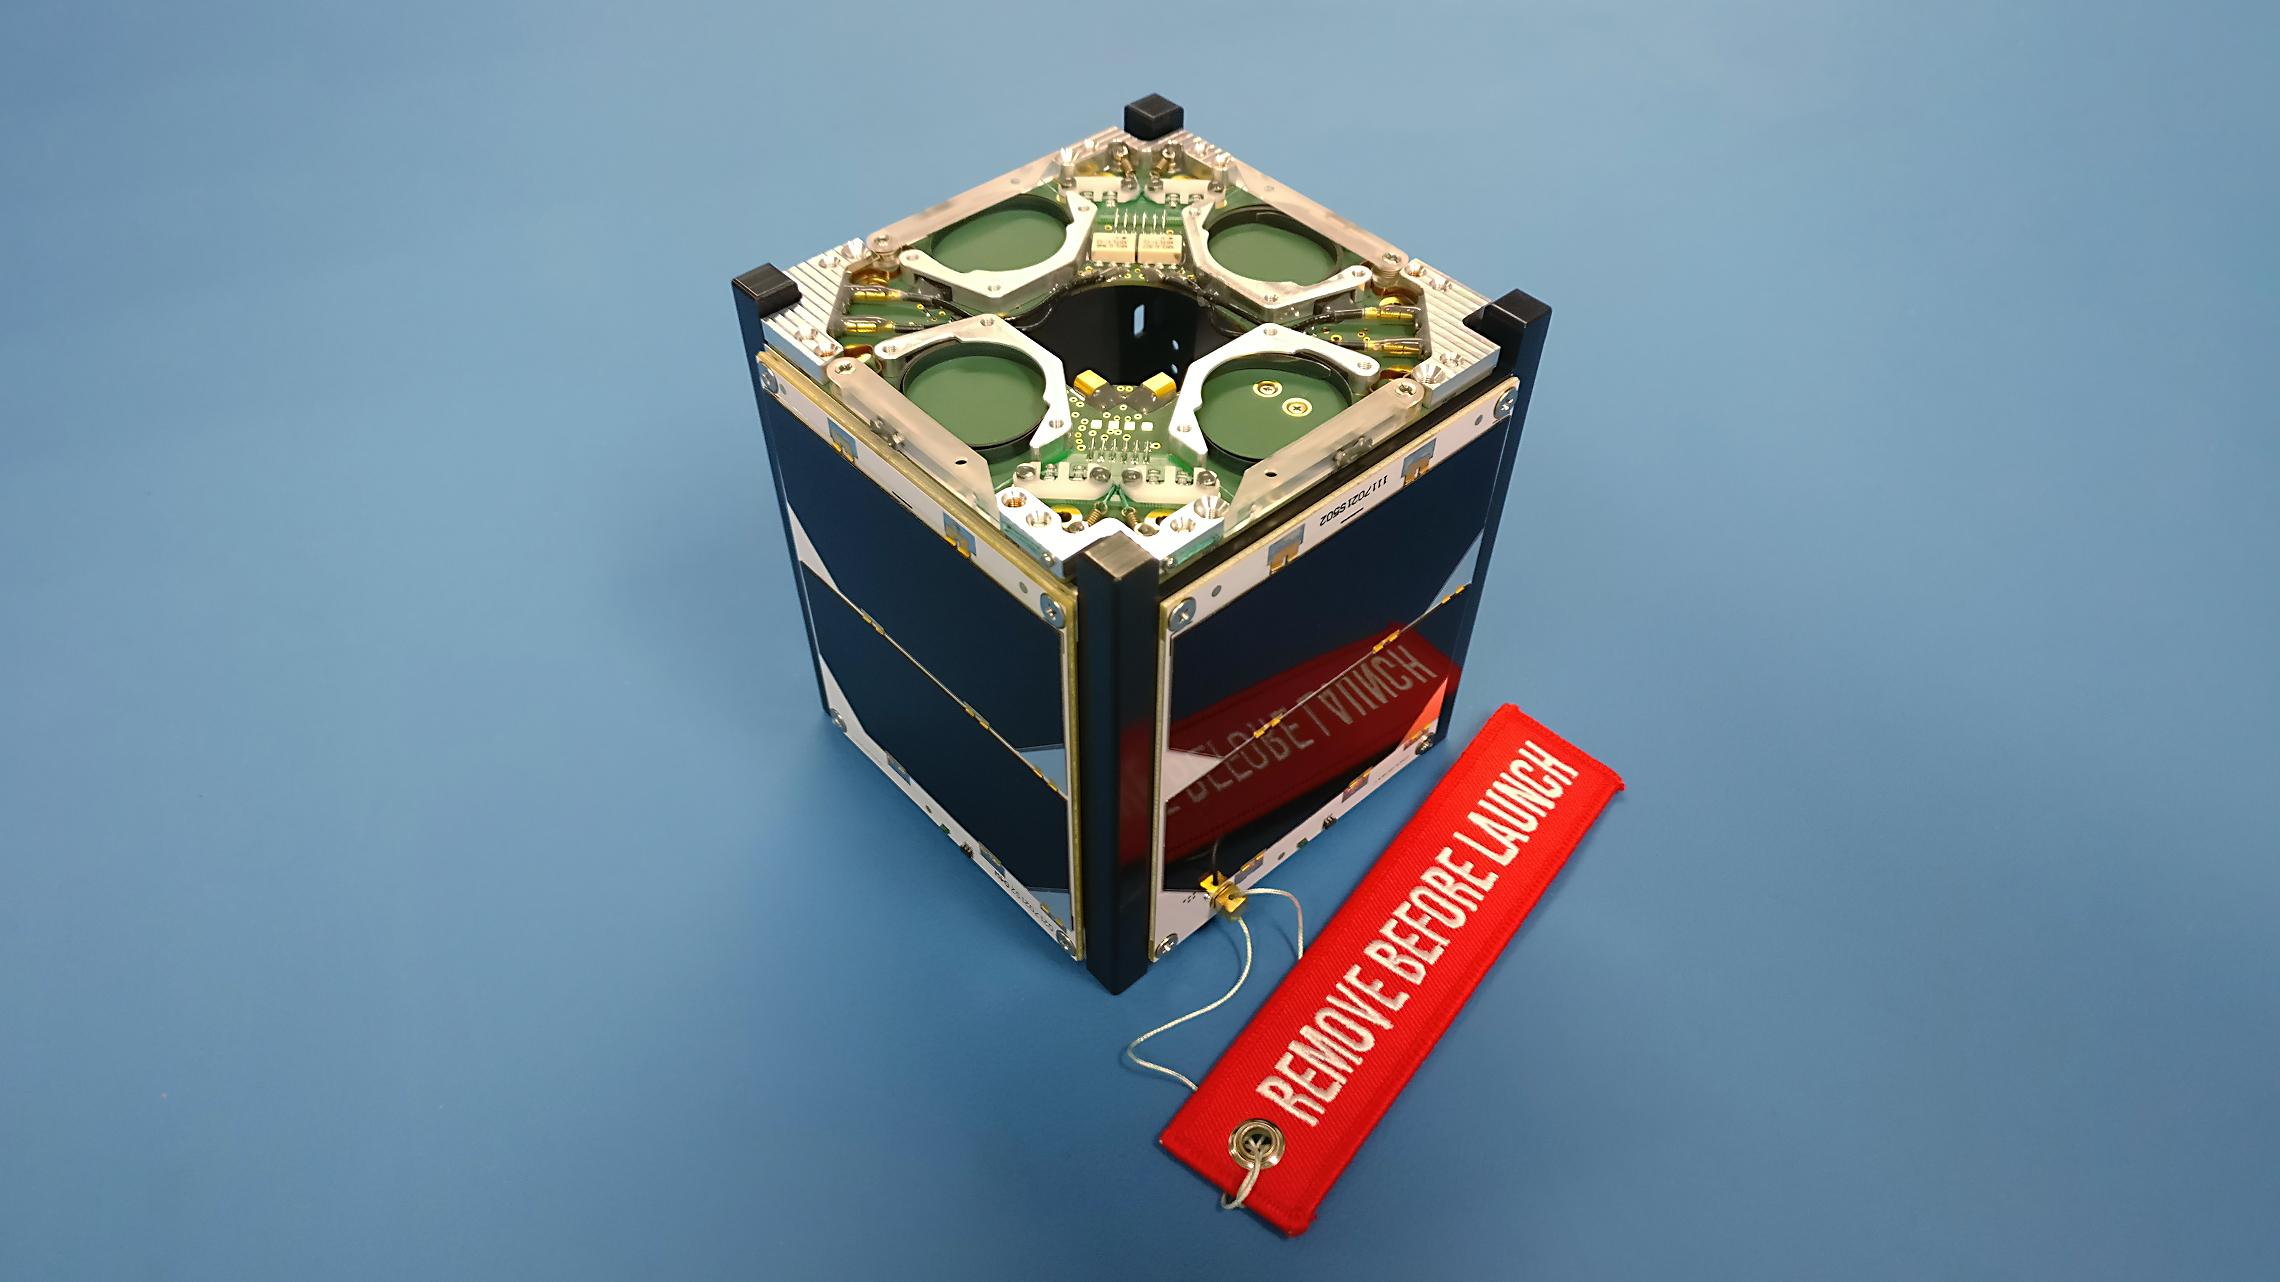
\includegraphics[width=.5\textwidth]{images/istsat1.jpeg}
	\caption[This piece of text is the image caption that will be shown in the list of tables at the start of the document.]{This piece of text will show up under the image itself. Having 2 different captions is useful when you want a long caption to appear next to the image itself since (as you can imagine) it won't look great to have a big description for a single figure in the list of figures.}
	\label{fig:normal_image}
\end{figure}

Figure \ref{fig:normal_image} shows a picture of ISTSat-1, a 1U CubeSat developed at Técnico. You can learn more about ISTSat-1 on \href{https://110.tecnico.ulisboa.pt/arquivos/episodio-34-istsat-1-o-1-o-cubesat-portugues/}{this} episode of the ``110 Histórias, 110 Objetos'' podcast or on the project's website: \url{https://istsat.one}.

What if you need something more difficult than just a single image? What if you need 2 images side by side? 

You can use the example code for Figure \ref{fig:subfigure_env} to have subcaptions for each of your subfigures and then a caption for both images.

%%%%%%%%%%%%%%%%%%%%%%%%% SUBFIGURE %%%%%%%%%%%%%%%%%%%%%%%%%
\begin{figure}[!htb]
    \centering
    \begin{subfigure}{.4\textwidth}
        \centering
        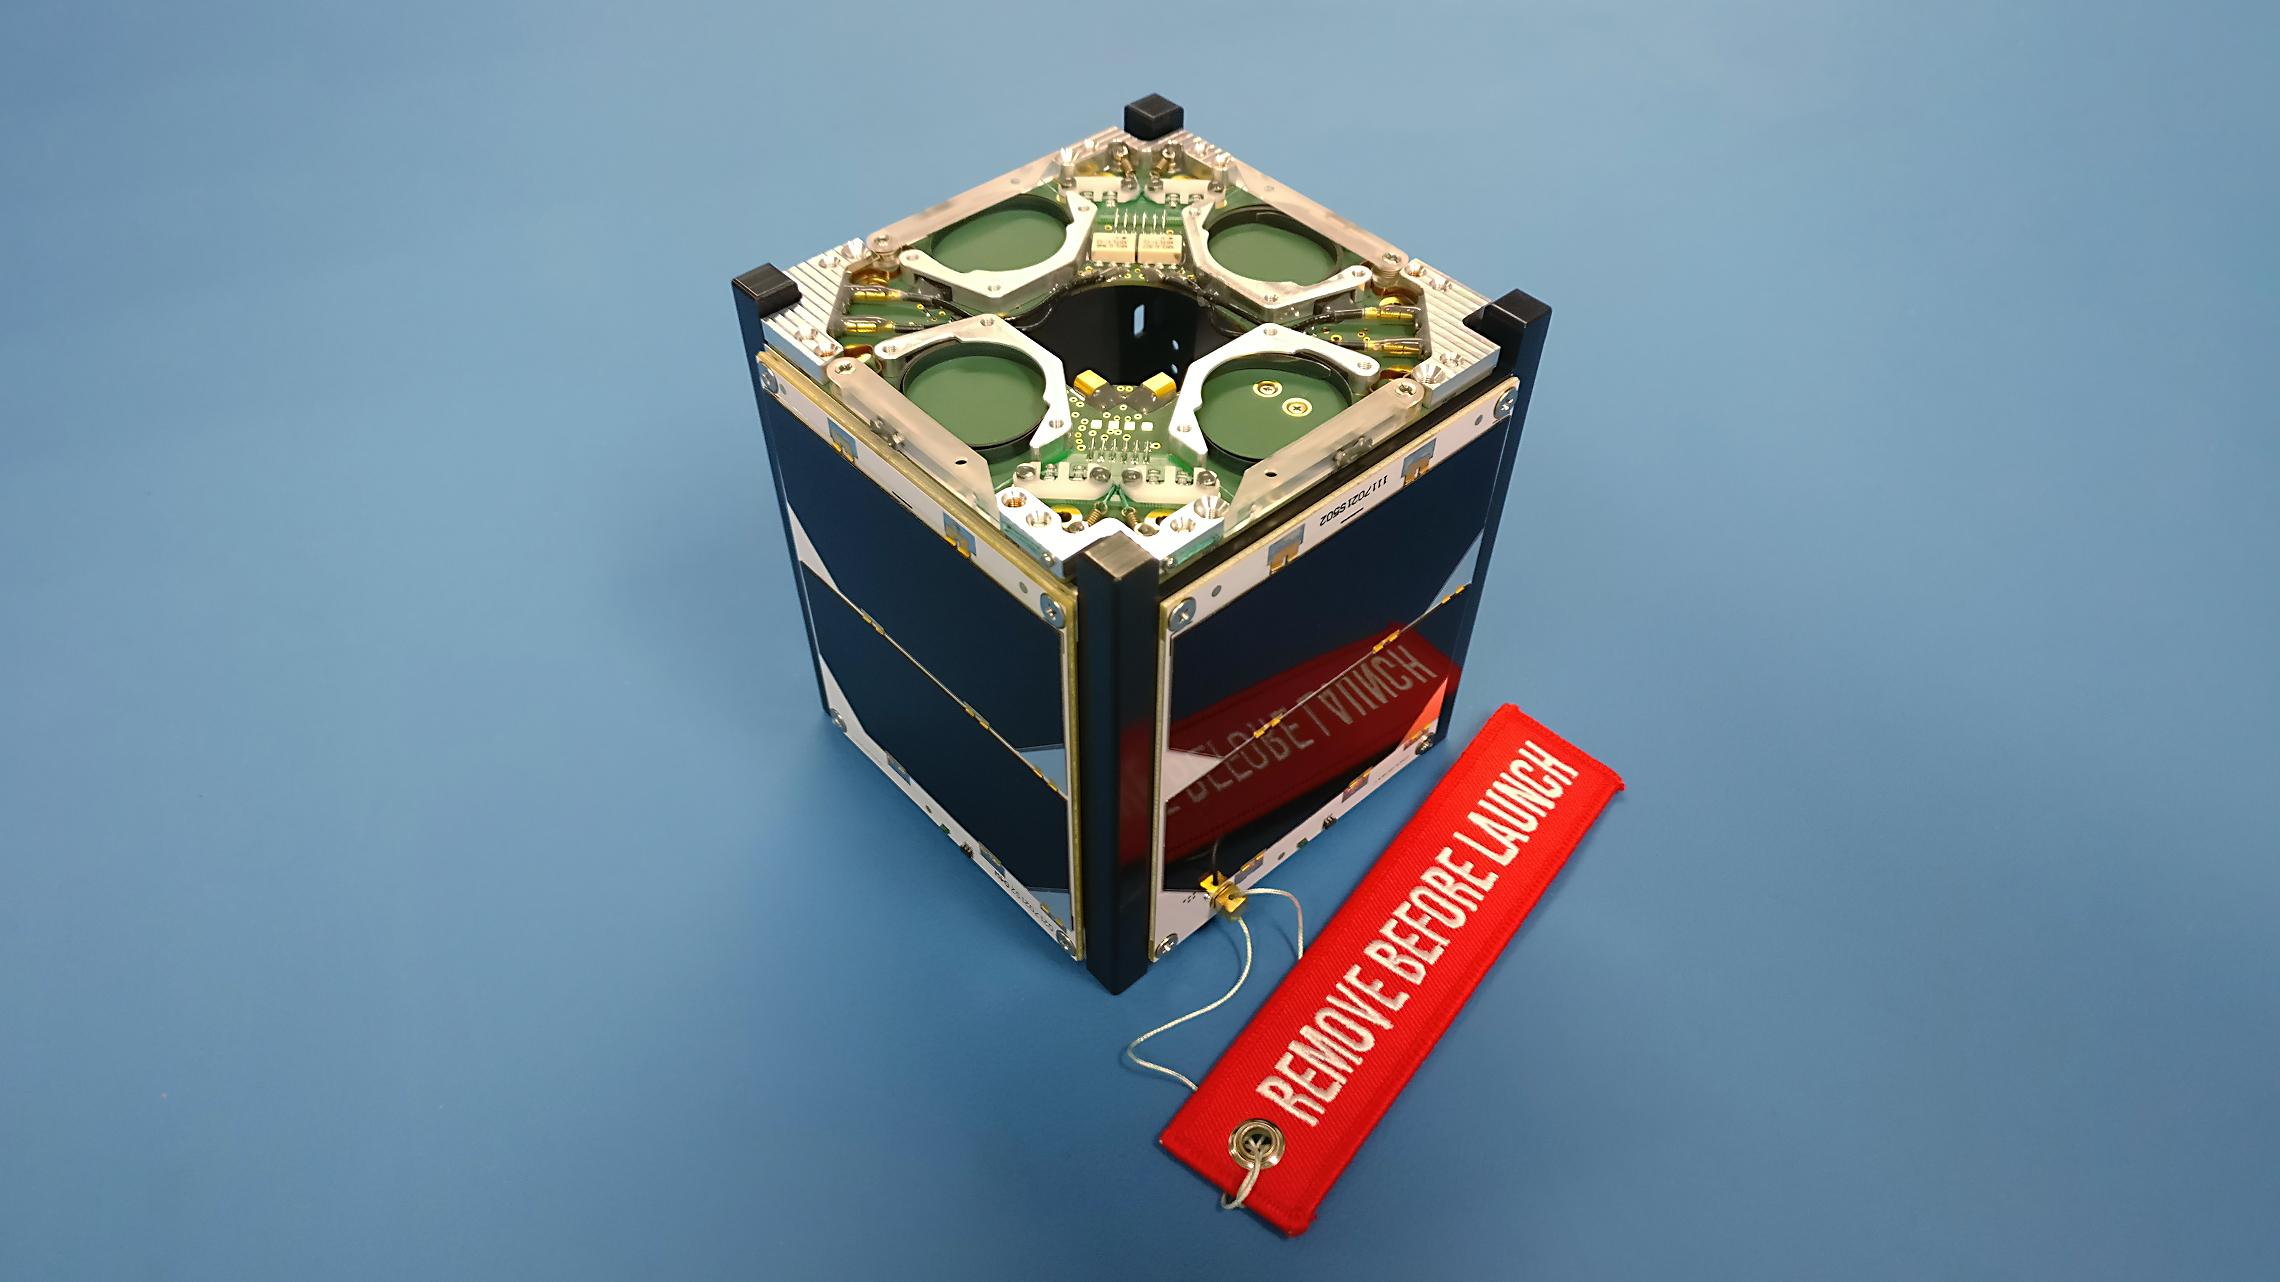
\includegraphics[width=\textwidth]{images/istsat1.jpeg}
        \caption{A caption.}
    \end{subfigure}
    \hfill
    \begin{subfigure}{.4\textwidth}
        \centering
        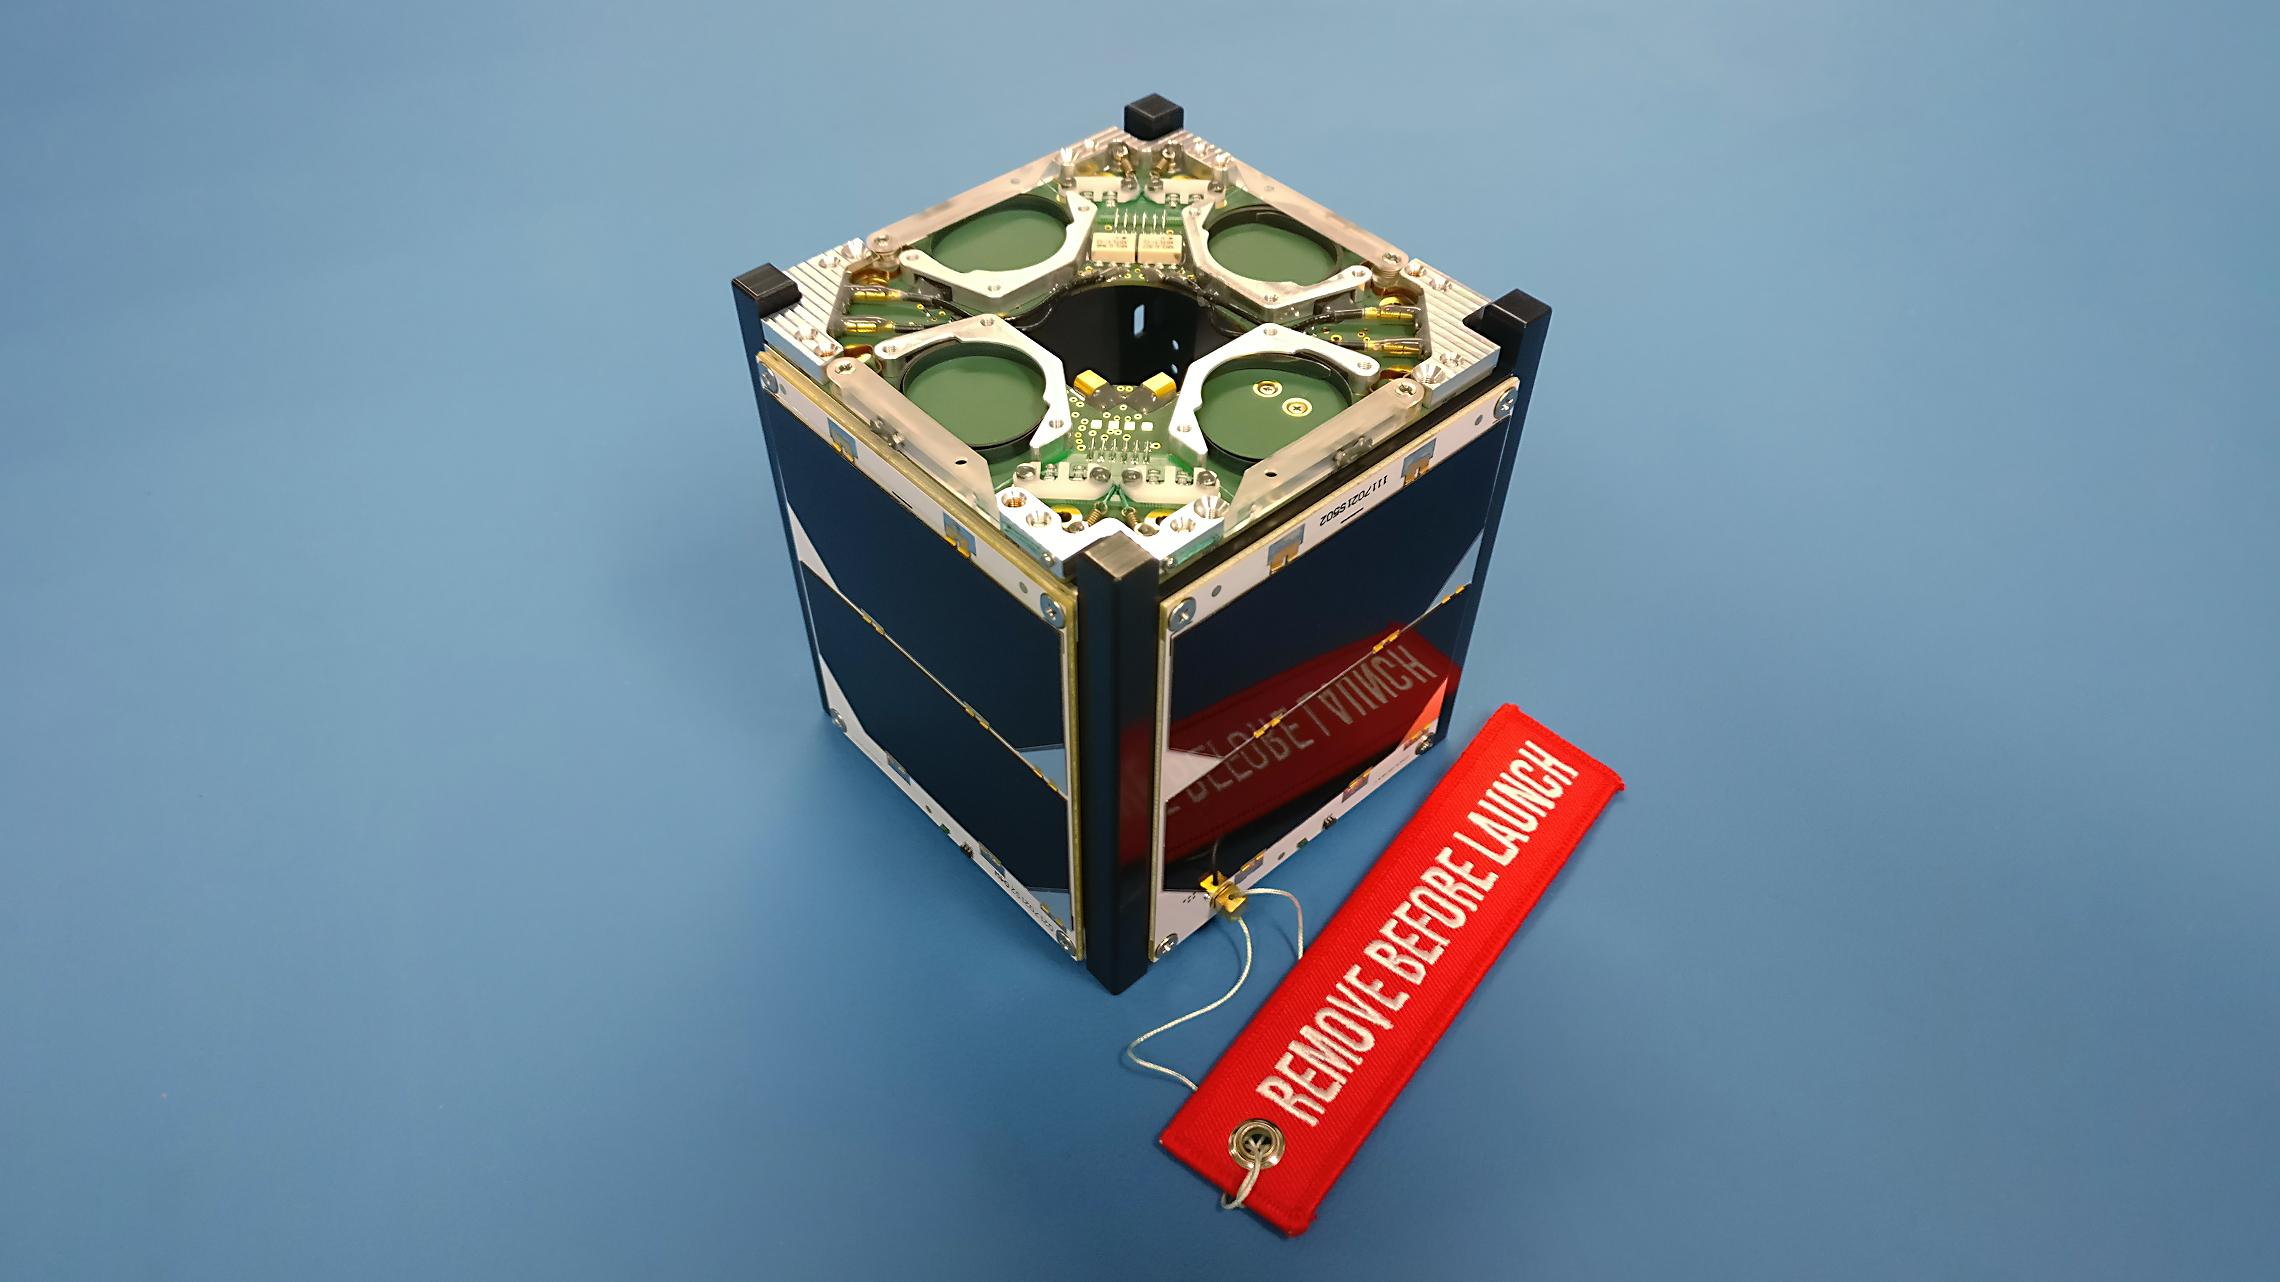
\includegraphics[width=\textwidth]{images/istsat1.jpeg}
        \caption{Another caption.}
    \end{subfigure}
    \caption{This example uses the subfigure environment. You can play with the space between images and image size by changing the percentages that are multiplied by ``textwidth'' for the images' widths.}
	\label{fig:subfigure_env}
\end{figure}

However, if yiu just want to have 2 completely independent images side-by-side, just use the example code for Figures \ref{fig:minipage_env_1} and \ref{fig:minipage_env_2}.

%%%%%%%%%%%%%%%%%%%%%%%%% MINIPAGE %%%%%%%%%%%%%%%%%%%%%%%%%
\begin{figure}[!htb]
    \centering
    \begin{minipage}{.45\linewidth}
        \centering
        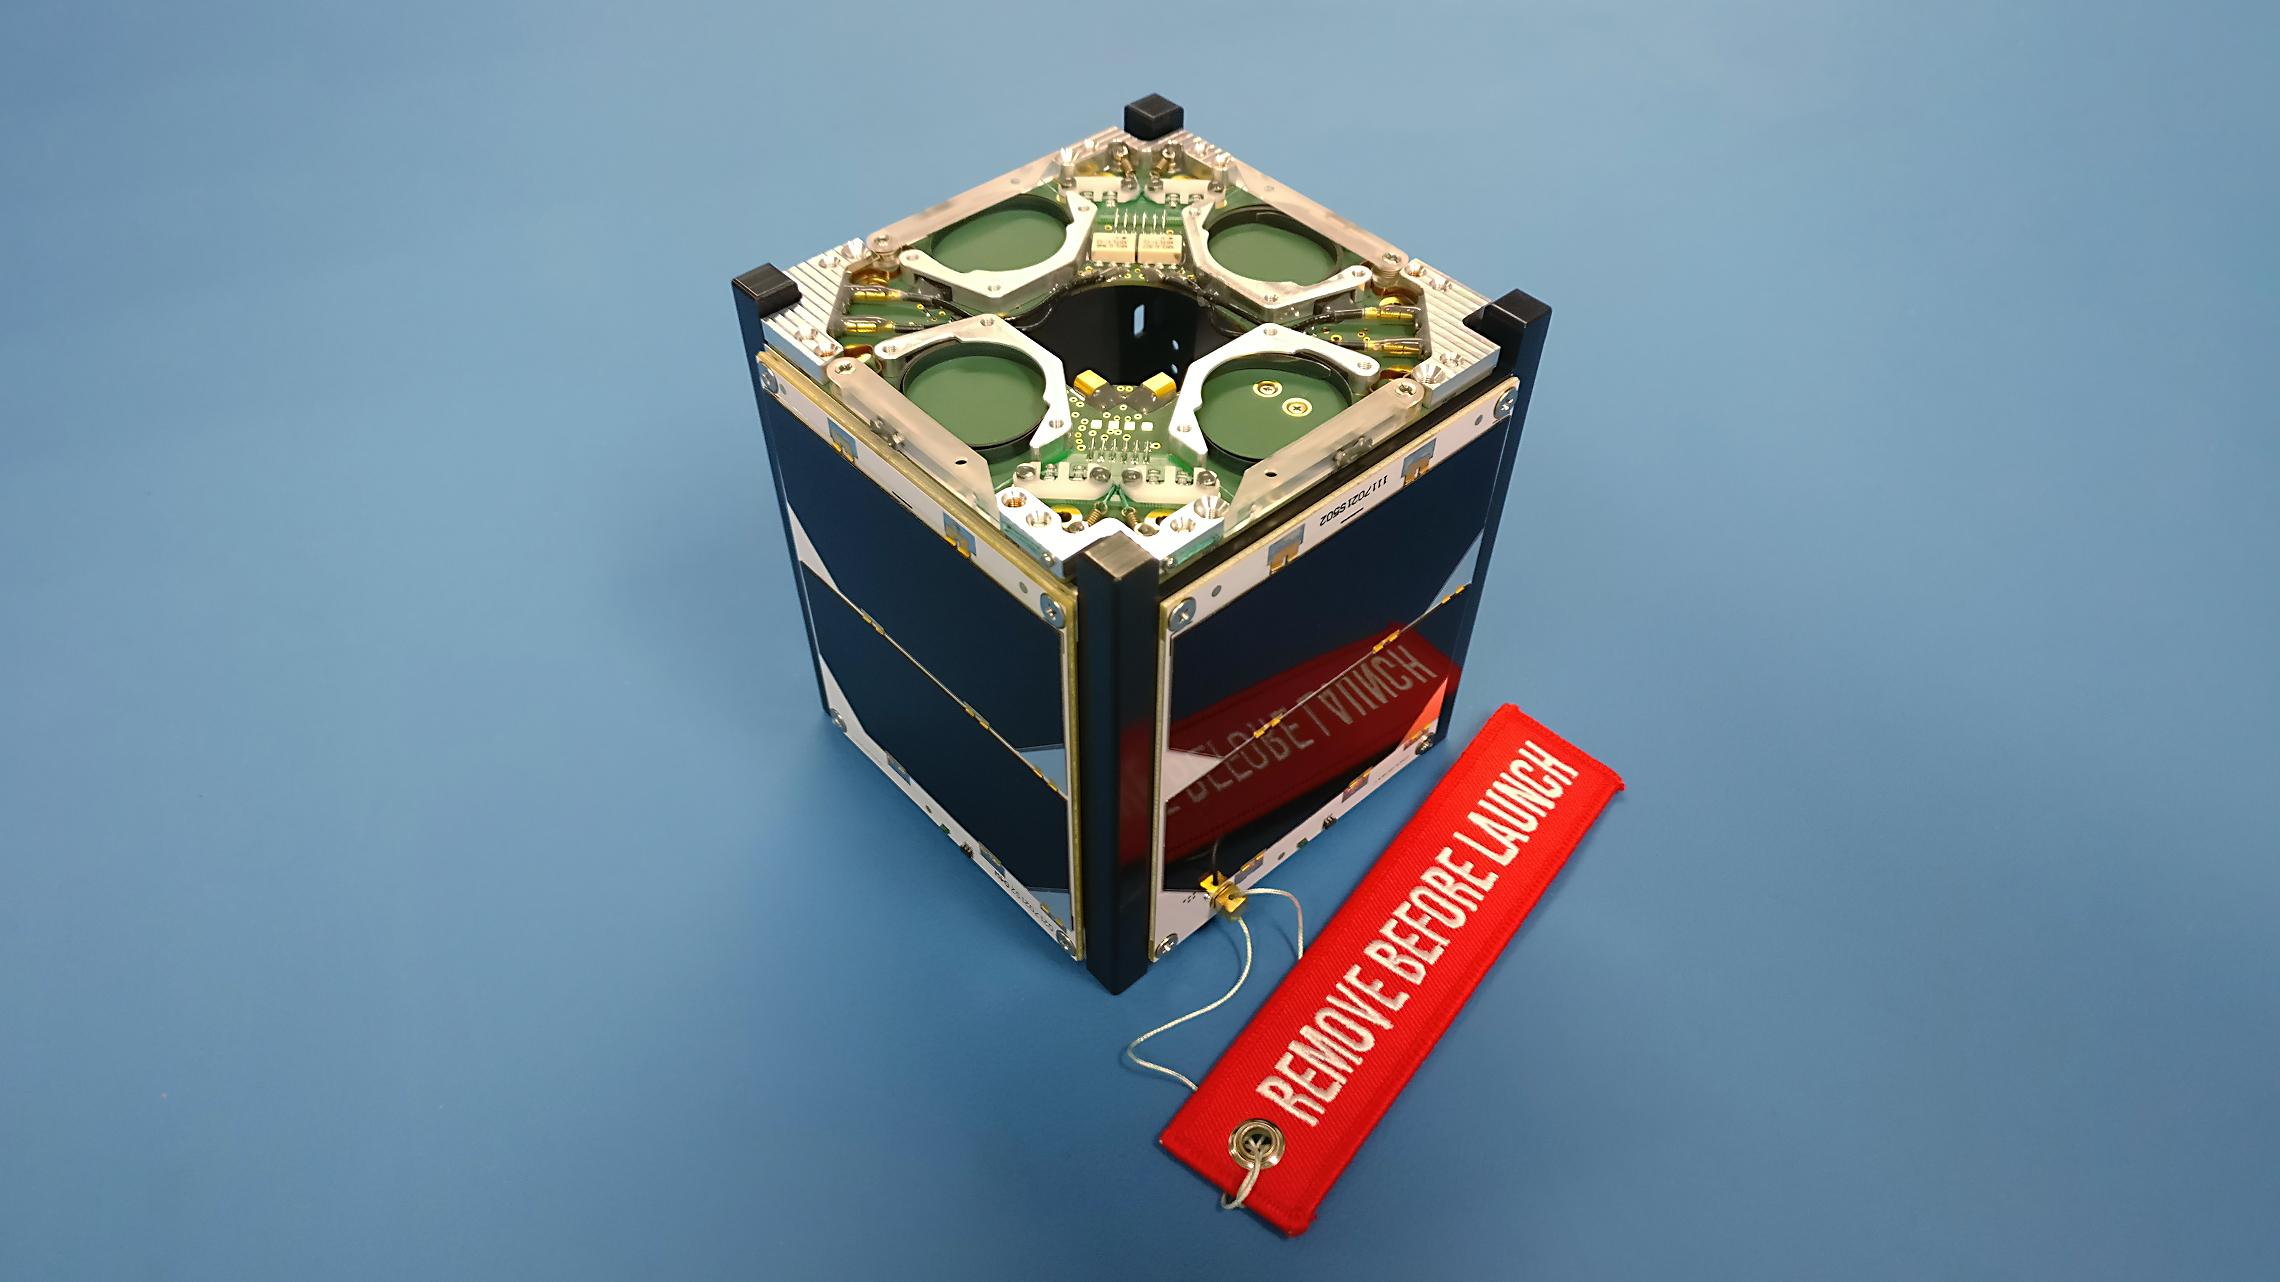
\includegraphics[width=0.6\textwidth]{images/istsat1.jpeg}
        \caption{An independent caption.}
		\label{fig:minipage_env_1}
    \end{minipage}
    \begin{minipage}{.45\linewidth}
        \centering
        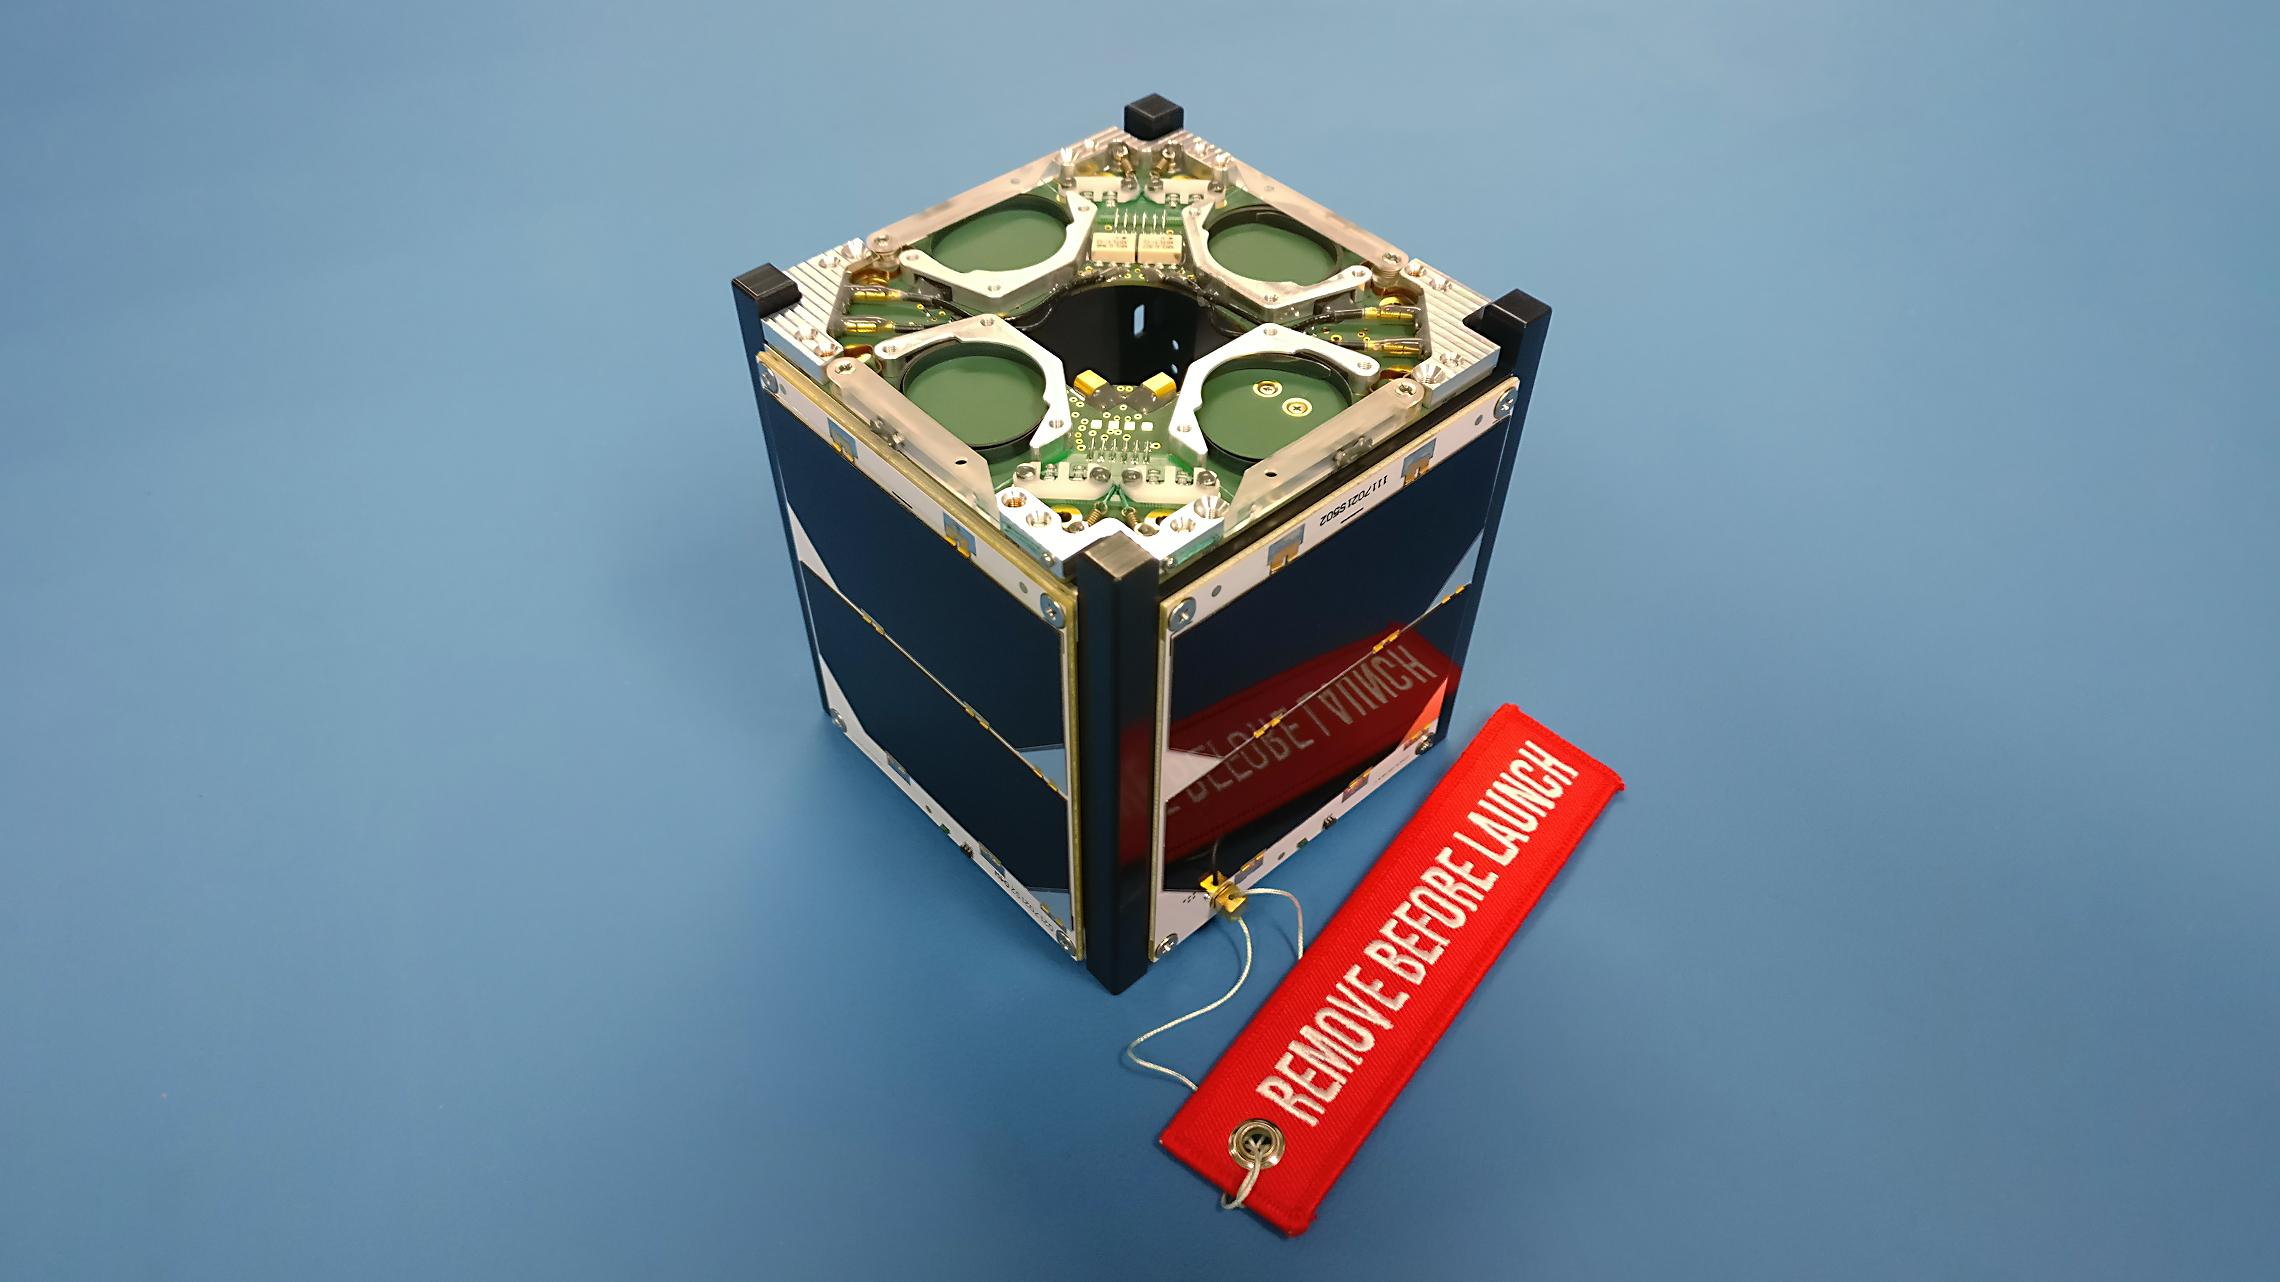
\includegraphics[width=0.6\textwidth]{images/istsat1.jpeg}
        \caption{Another independent caption.}
		\label{fig:minipage_env_2}
    \end{minipage}
\end{figure}

What if you need more than 2 images side by side? Follow the example of Figures \ref{fig:four_in_row_1}, \ref{fig:four_in_row_2}, \ref{fig:four_in_row_3} and \ref{fig:four_in_row_4}.

\begin{figure}[!htb]
    \centering
    \begin{minipage}{.2\linewidth}
        \centering
        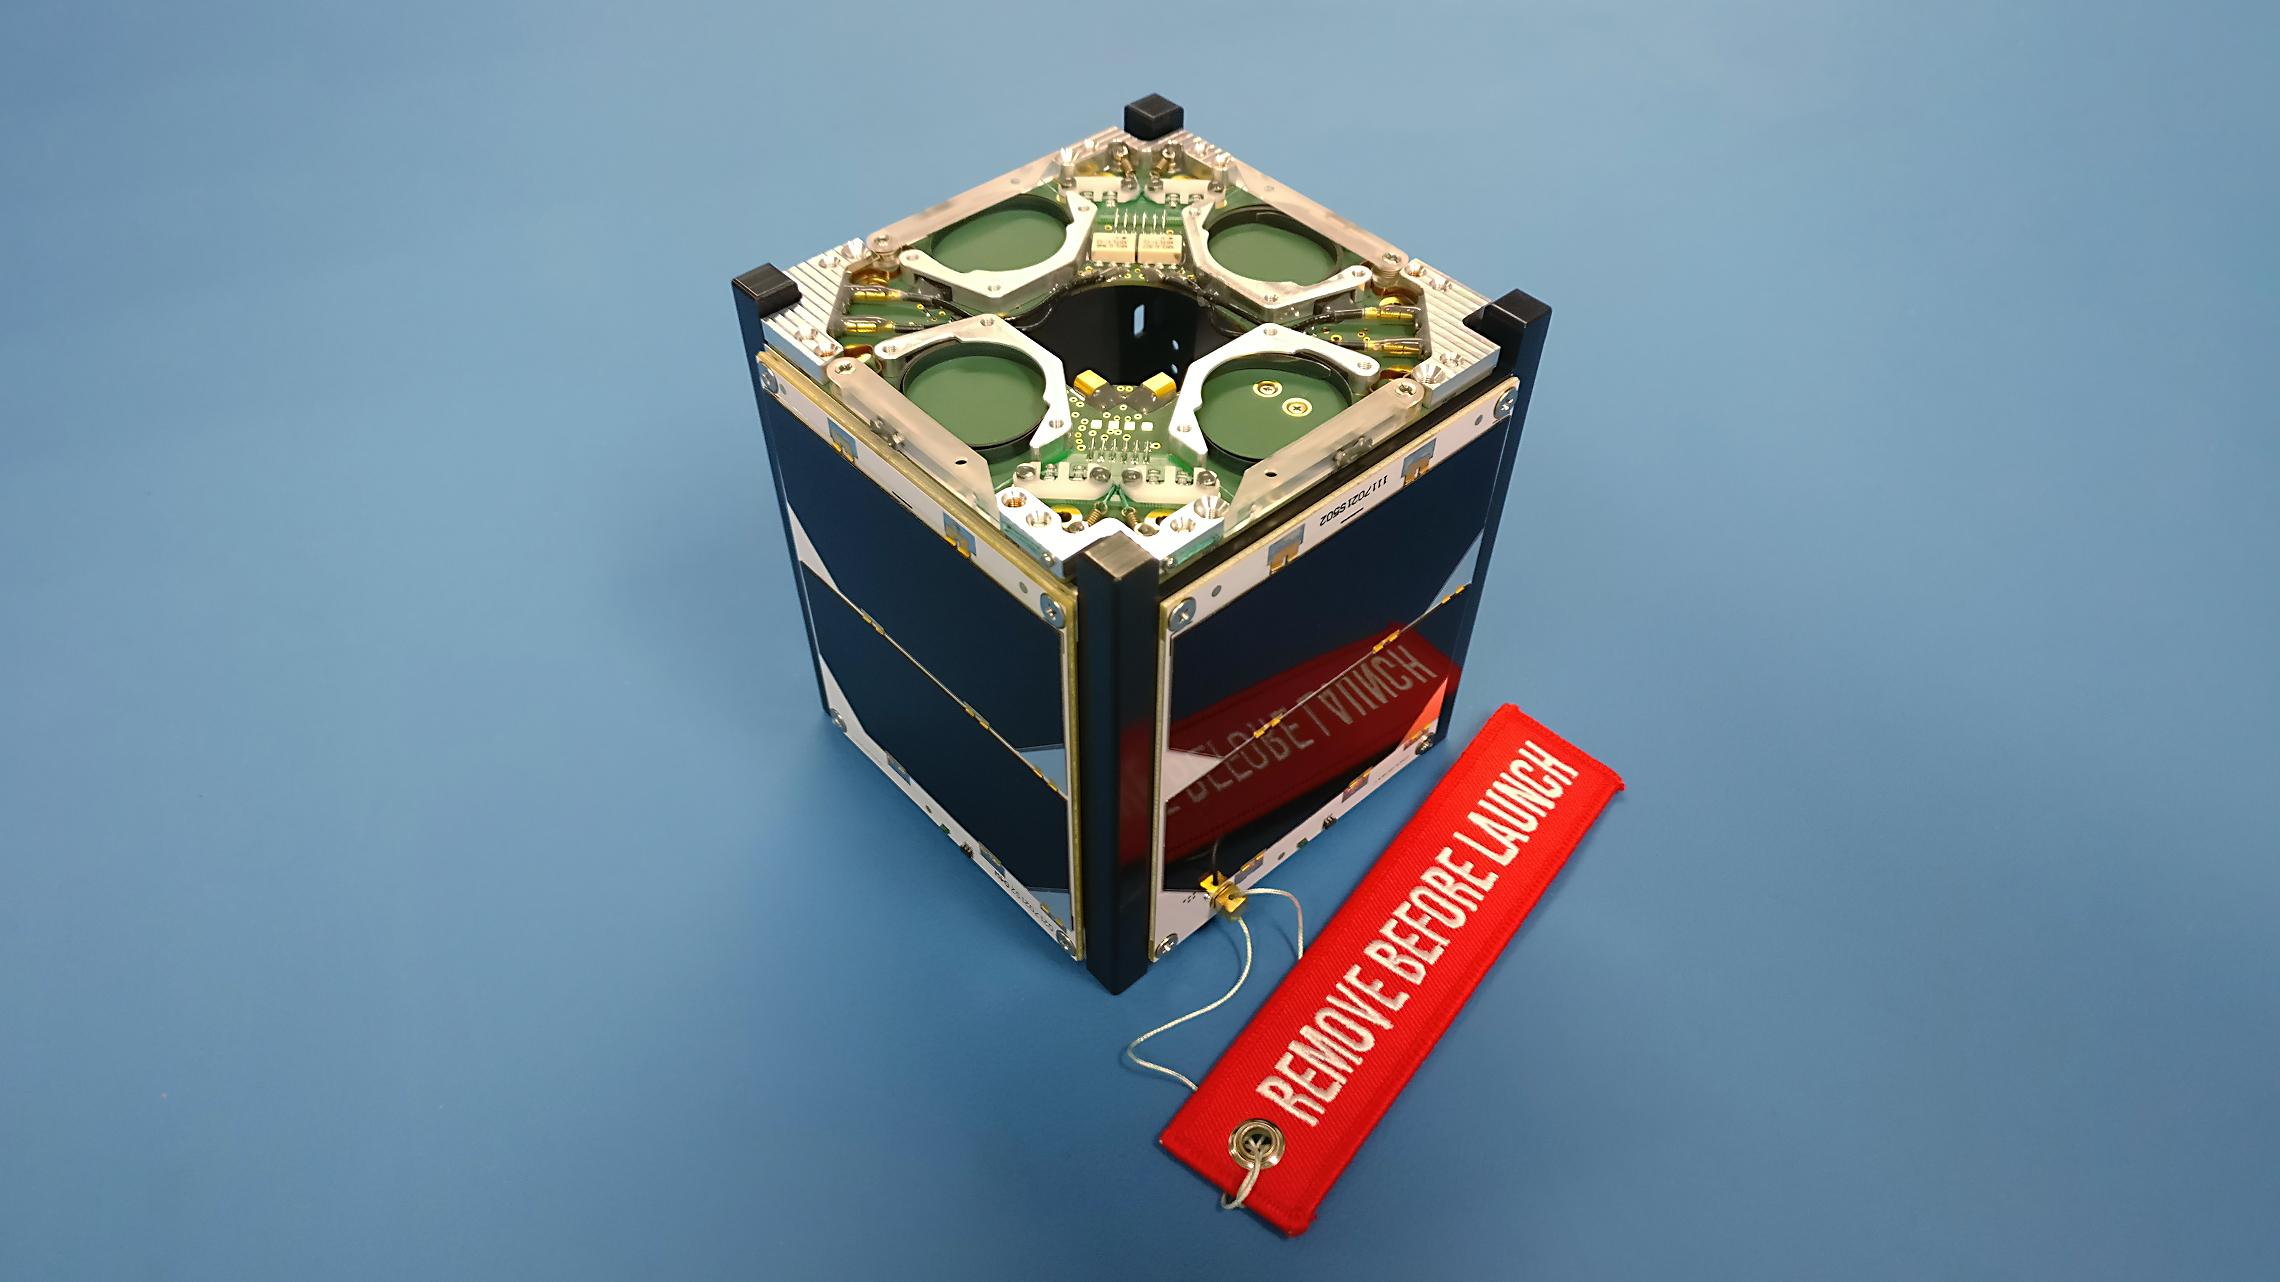
\includegraphics[width=0.95\textwidth]{images/istsat1.jpeg}
        \caption{An independent caption.}
		\label{fig:four_in_row_1}
    \end{minipage}
    \begin{minipage}{.2\linewidth}
        \centering
        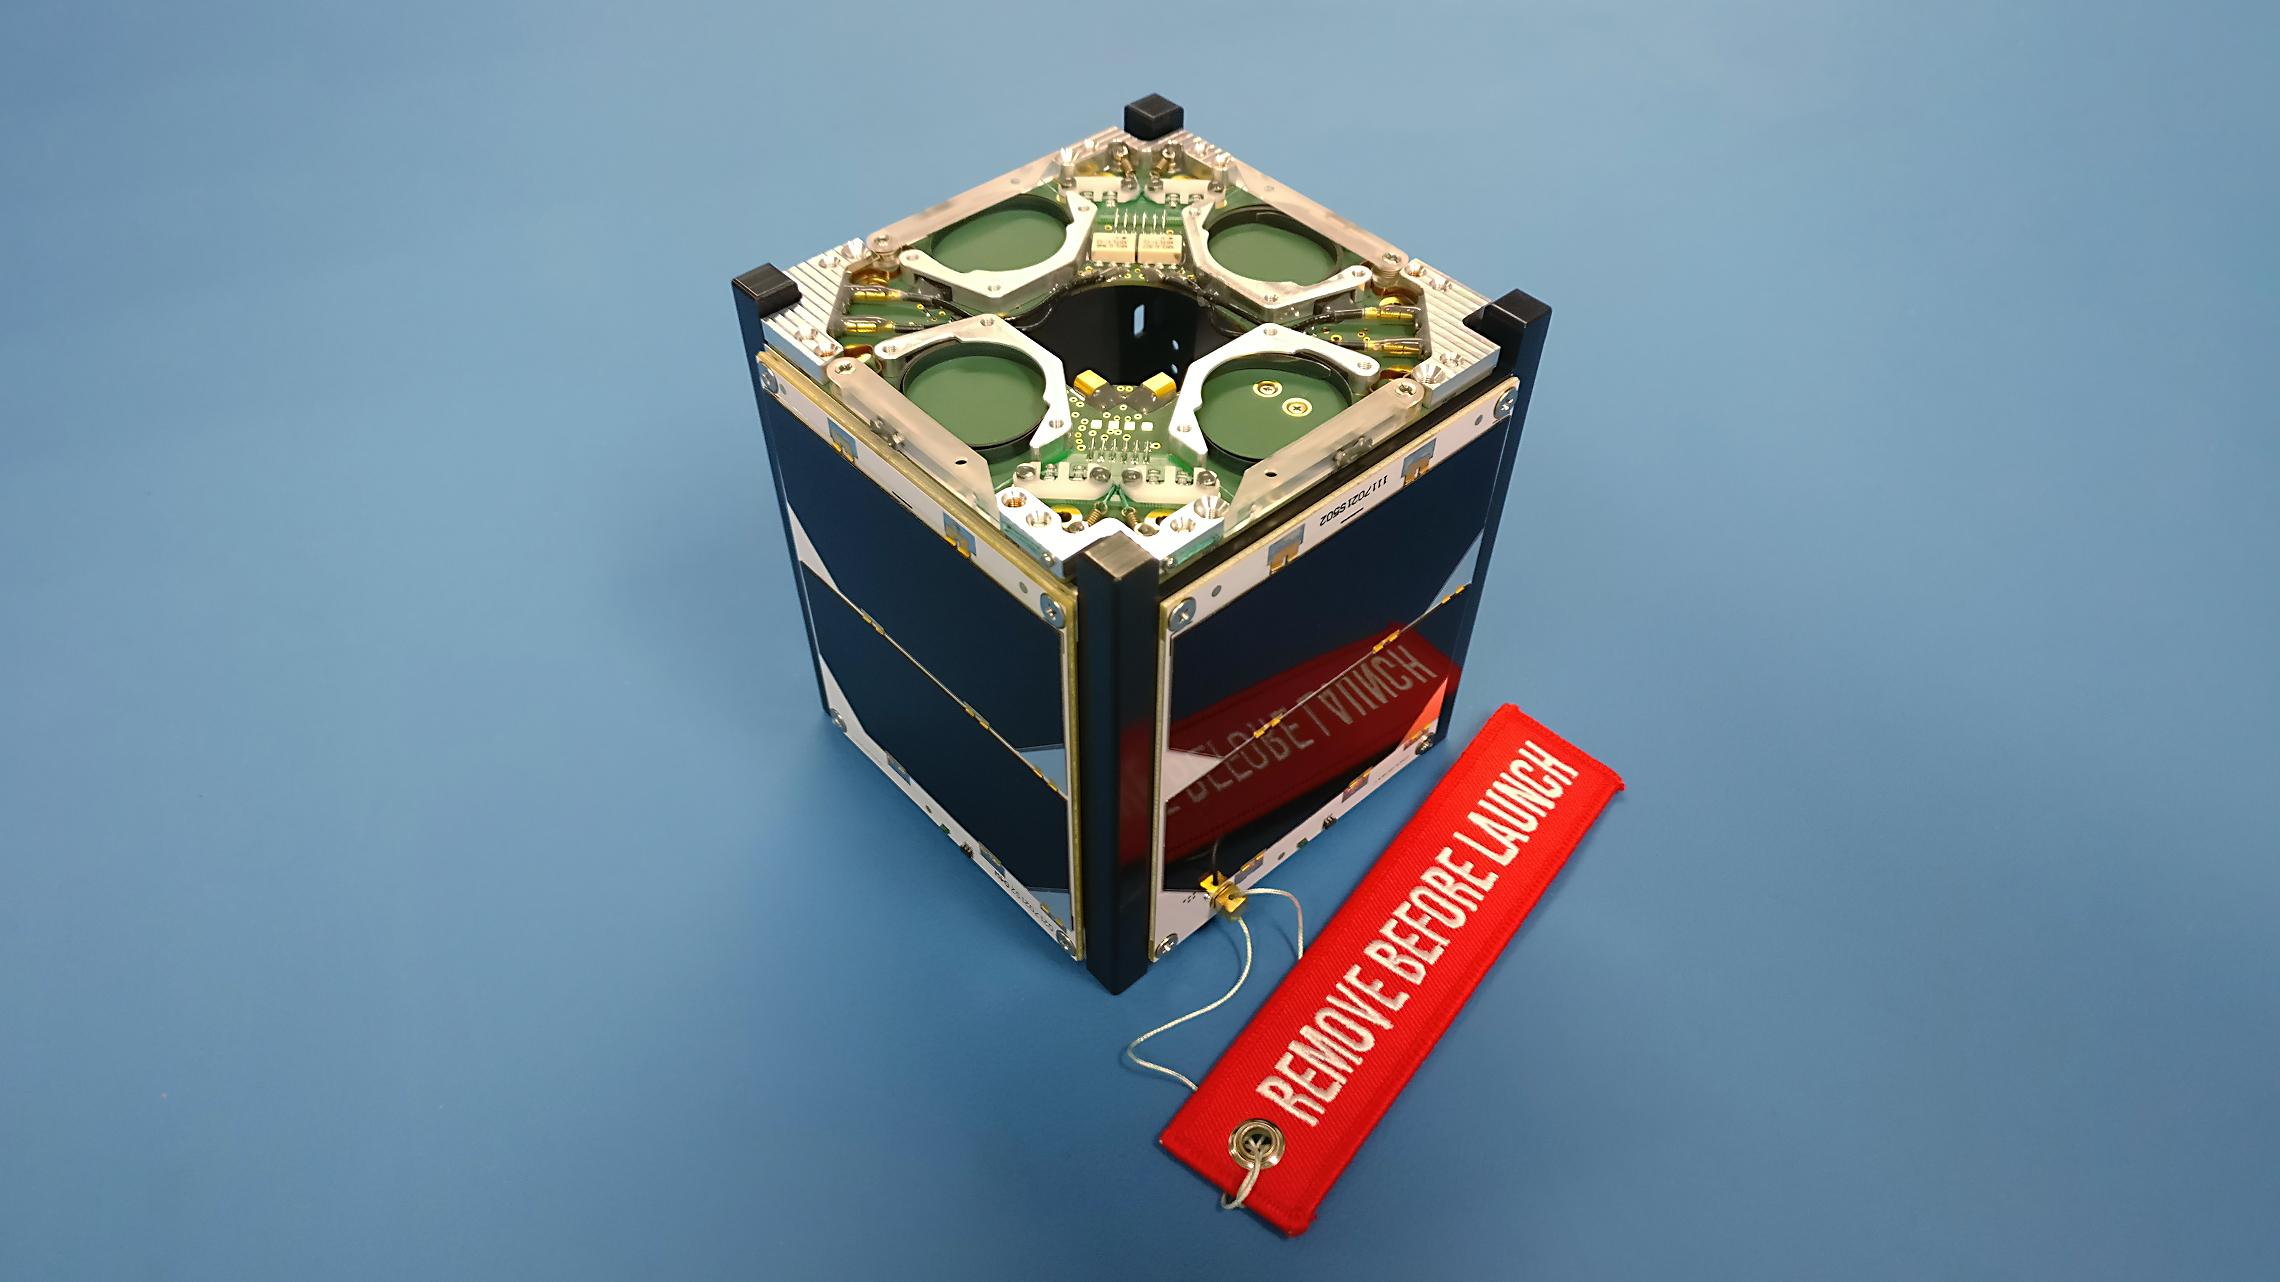
\includegraphics[width=0.95\textwidth]{images/istsat1.jpeg}
        \caption{Another independent caption.}
		\label{fig:four_in_row_2}
    \end{minipage}
	\begin{minipage}{.2\linewidth}
        \centering
        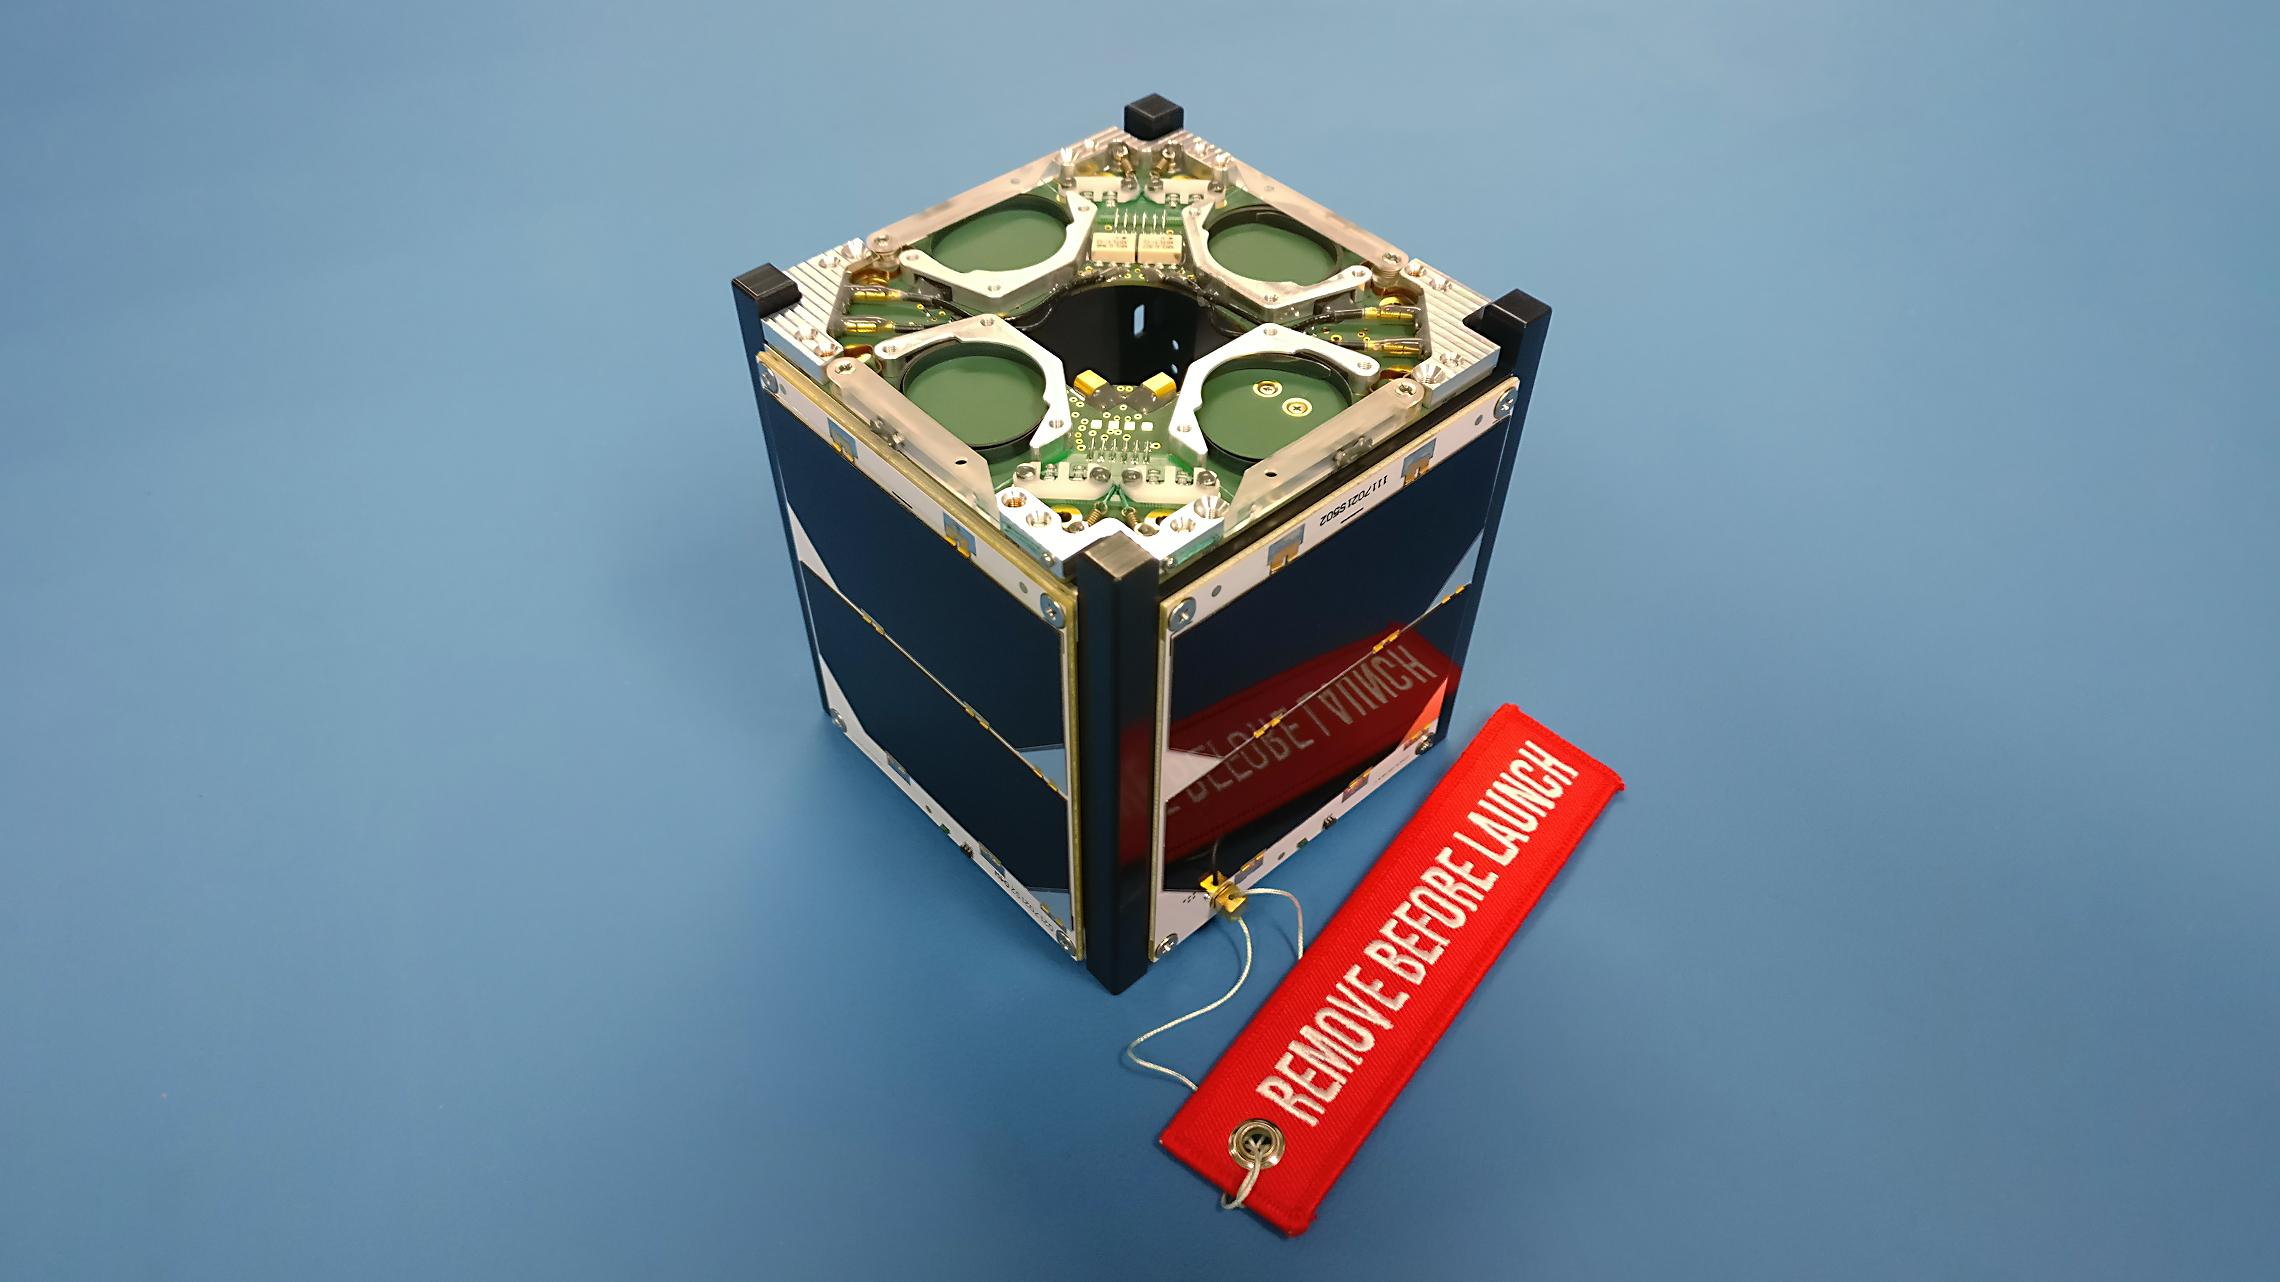
\includegraphics[width=0.95\textwidth]{images/istsat1.jpeg}
        \caption{Another independent caption.}
		\label{fig:four_in_row_3}
    \end{minipage}
	\begin{minipage}{.2\linewidth}
        \centering
        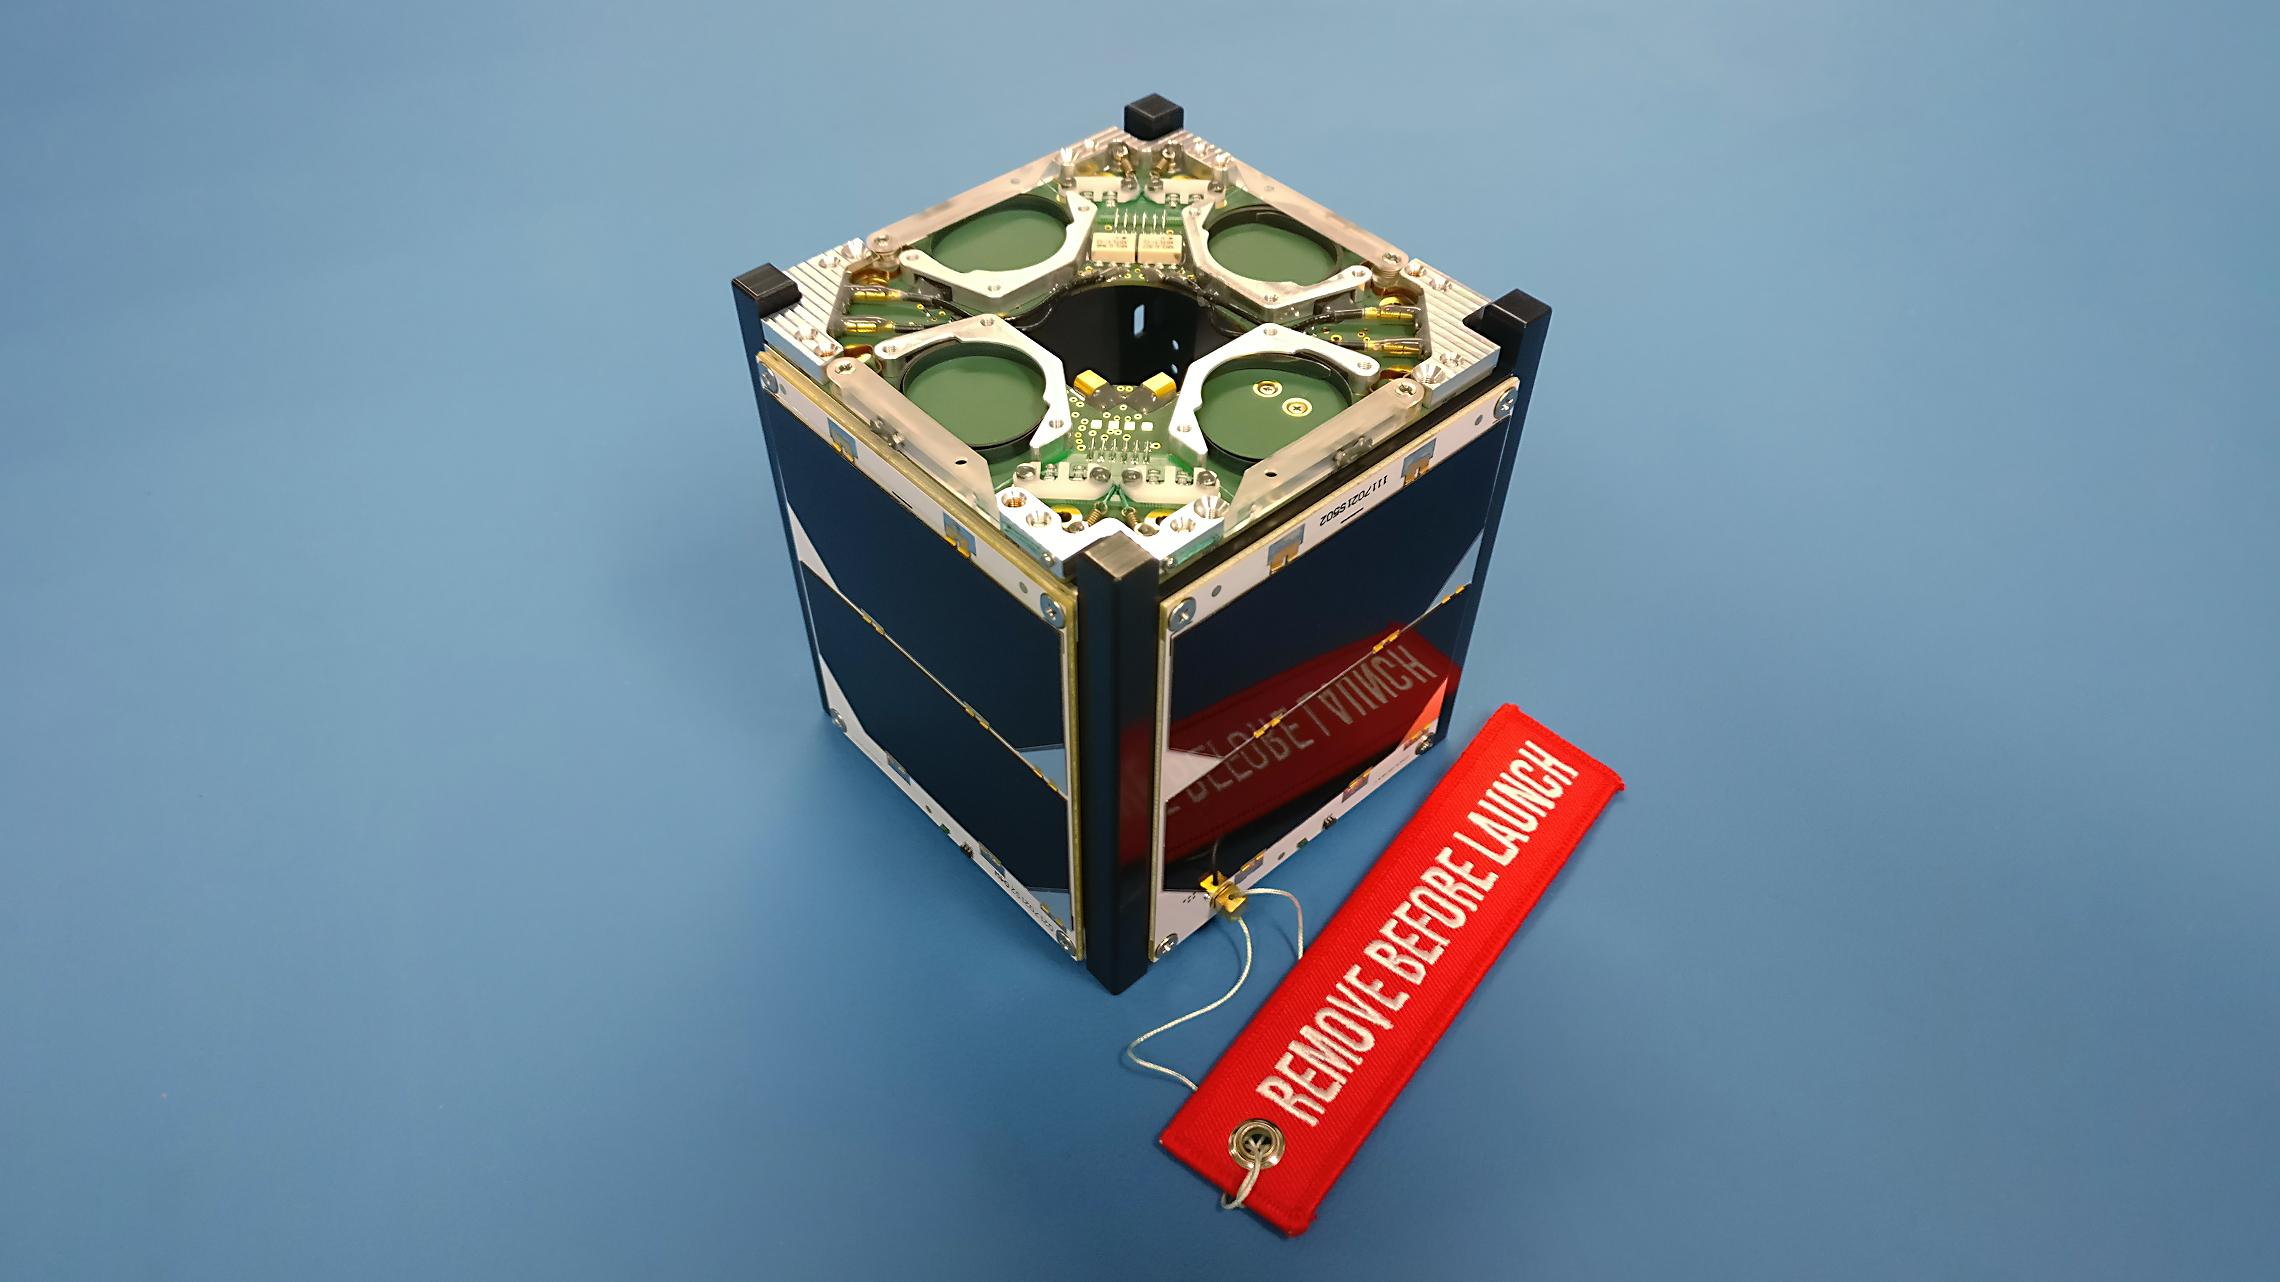
\includegraphics[width=0.95\textwidth]{images/istsat1.jpeg}
        \caption{Another independent caption.}
		\label{fig:four_in_row_4}
    \end{minipage}
\end{figure}

For more than 1 row of figures follow the example of Figure \ref{fig:five_images}.

\begin{figure}[!htb]
	\centering

    \begin{subfigure}[t]{0.3\textwidth}
        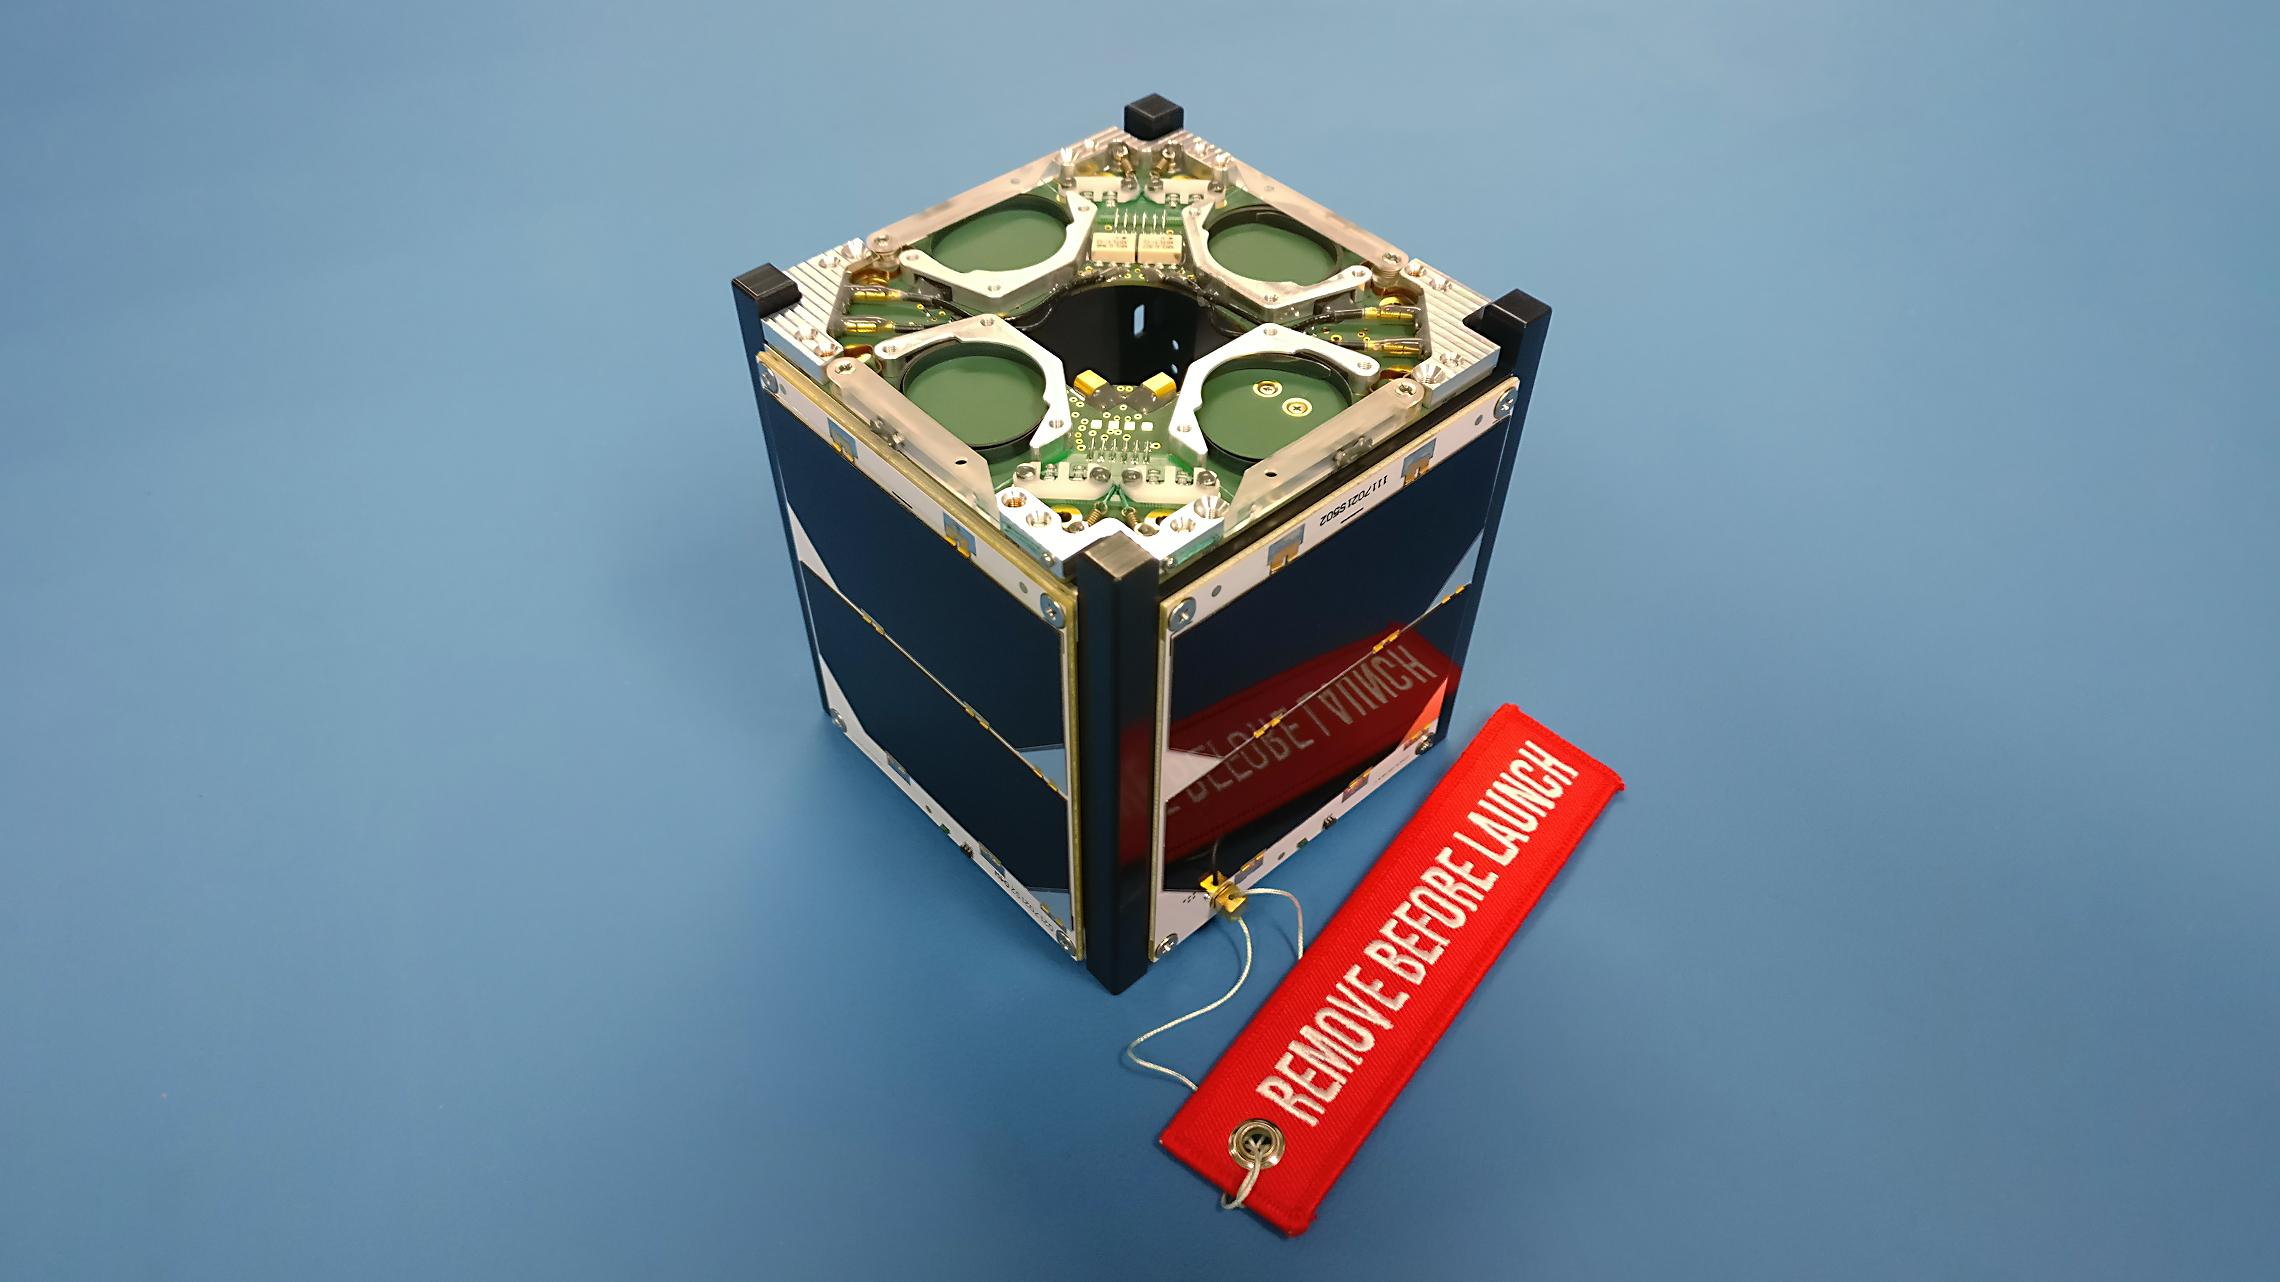
\includegraphics[width=\linewidth]{images/istsat1.jpeg}
		\caption{A caption.}
    \end{subfigure}
	\hfill
    \begin{subfigure}[t]{0.3\textwidth}
        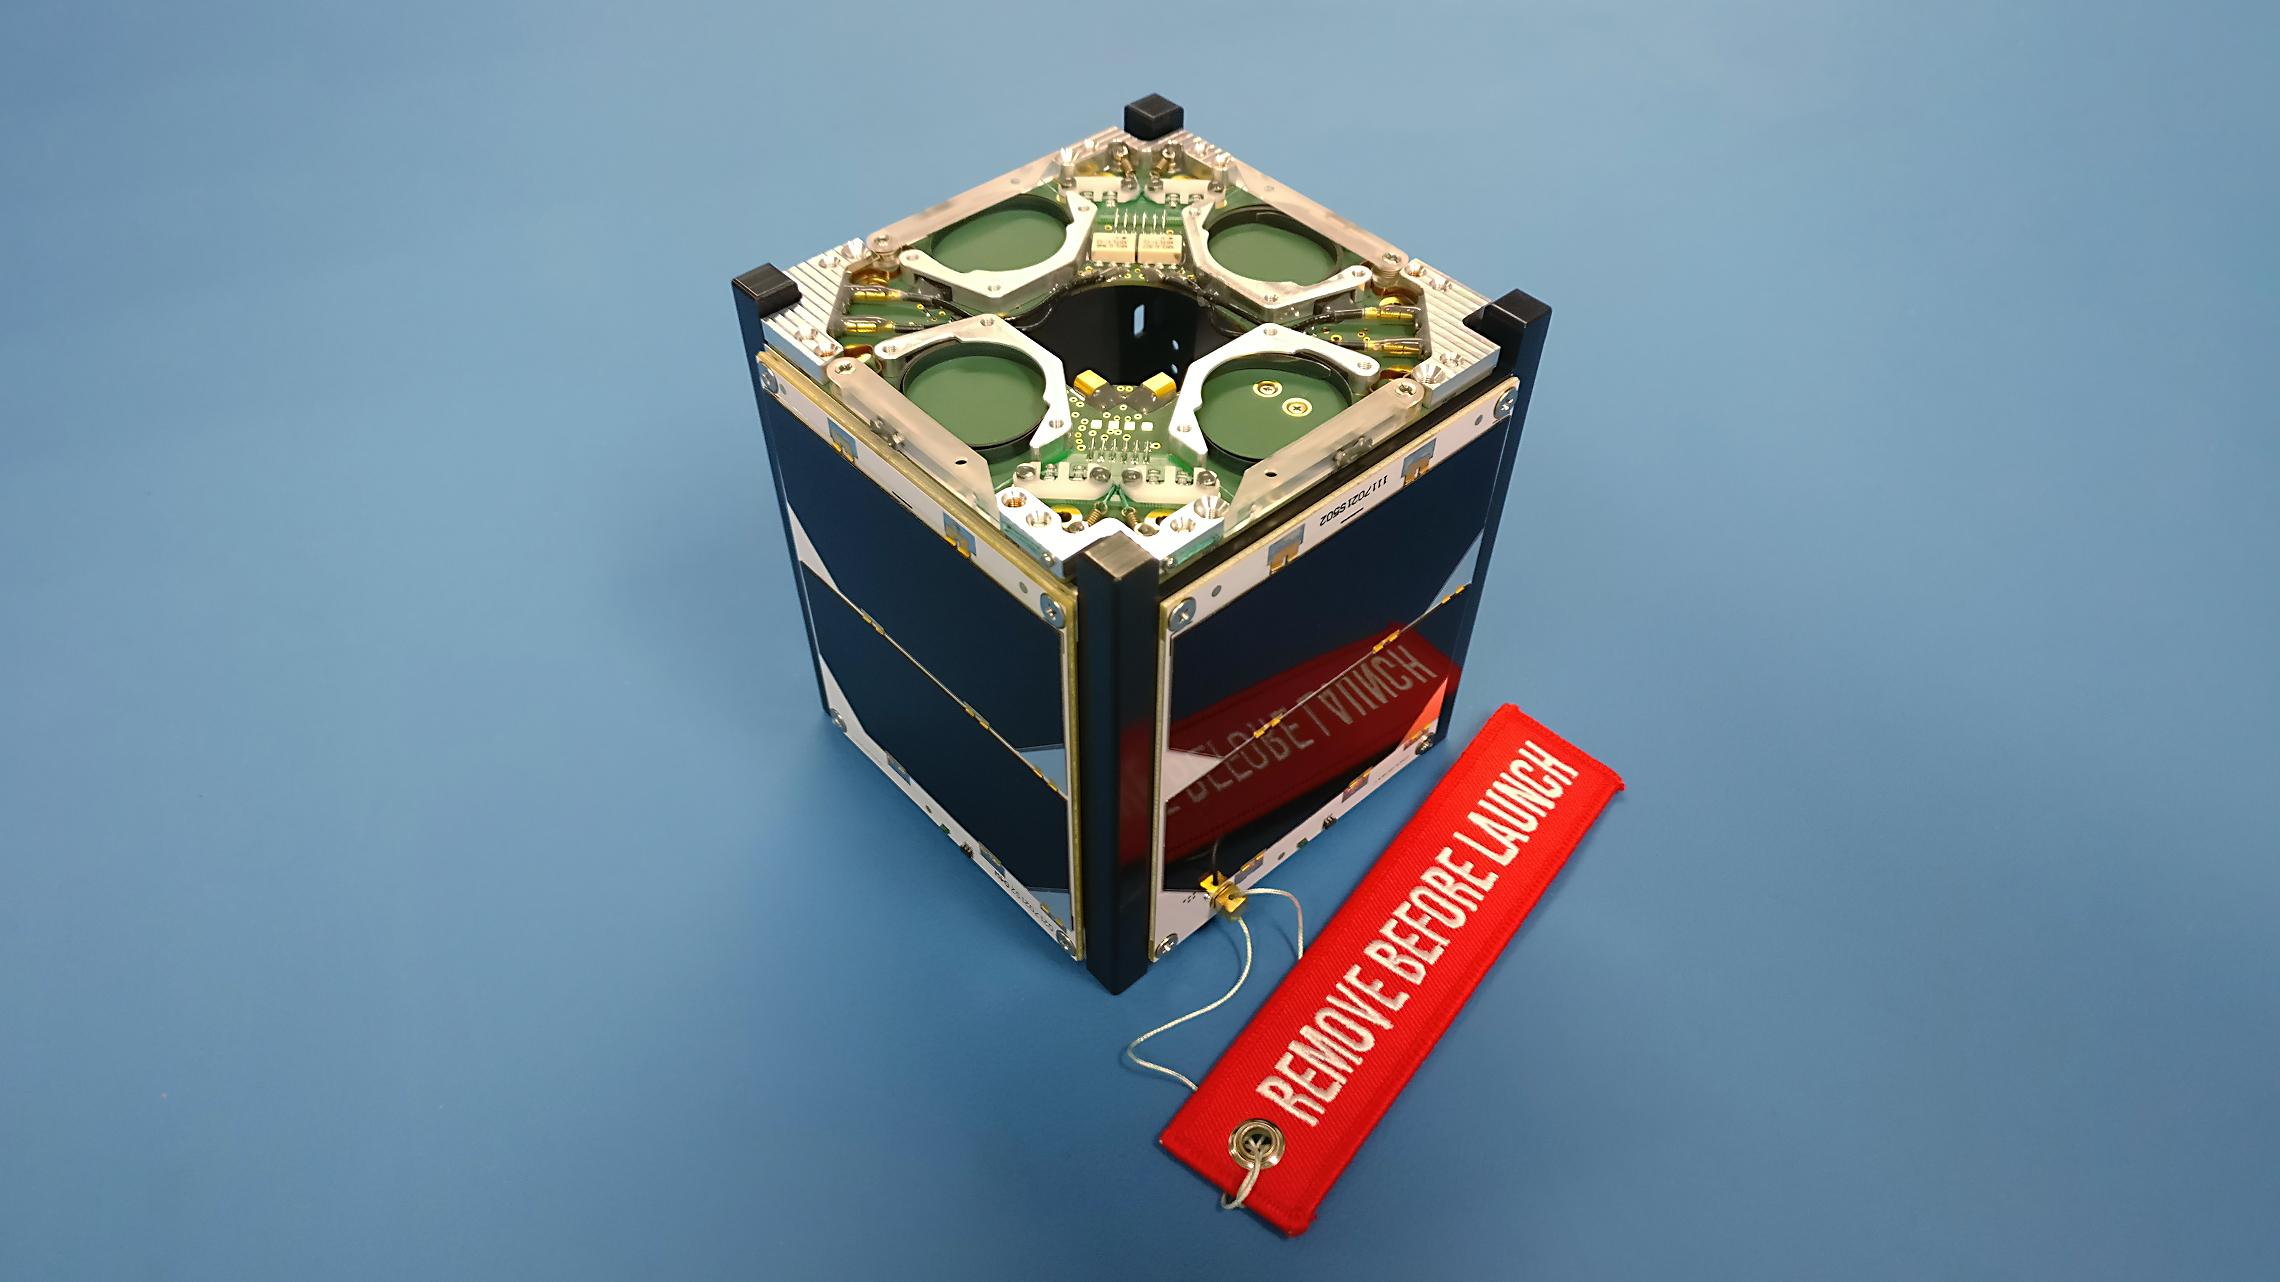
\includegraphics[width=\linewidth]{images/istsat1.jpeg}
		\caption{A caption.}
    \end{subfigure}
	\hfill
    \begin{subfigure}[t]{0.3\textwidth}
        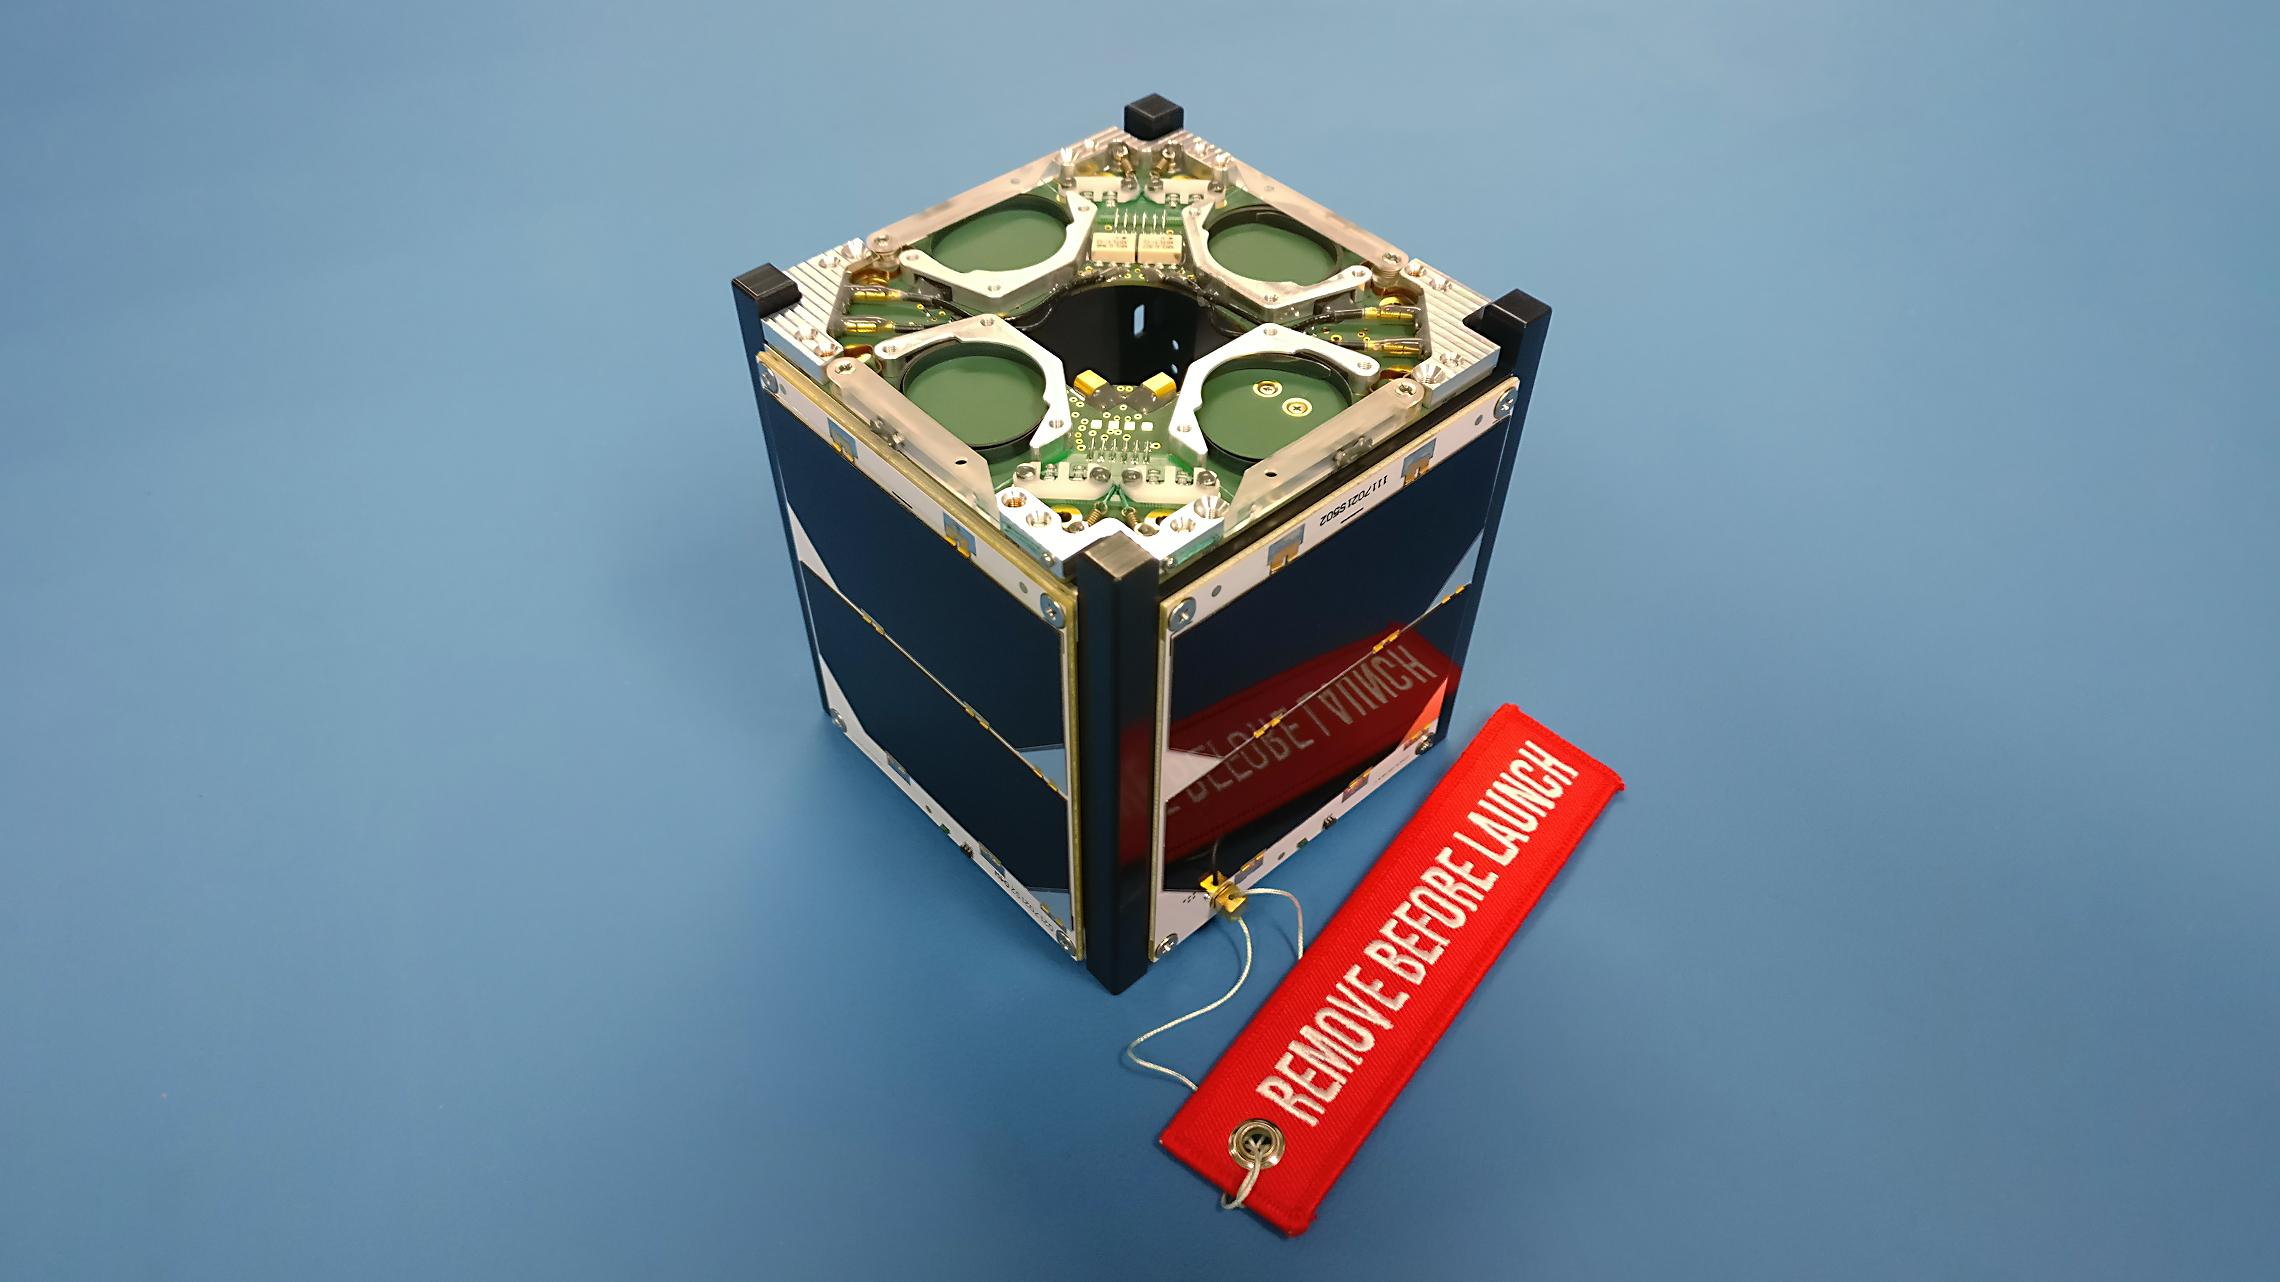
\includegraphics[width=\linewidth]{images/istsat1.jpeg}
		\caption{A caption.}
    \end{subfigure}

	\vspace{0.4cm}

    \begin{subfigure}[t]{0.3\textwidth}
        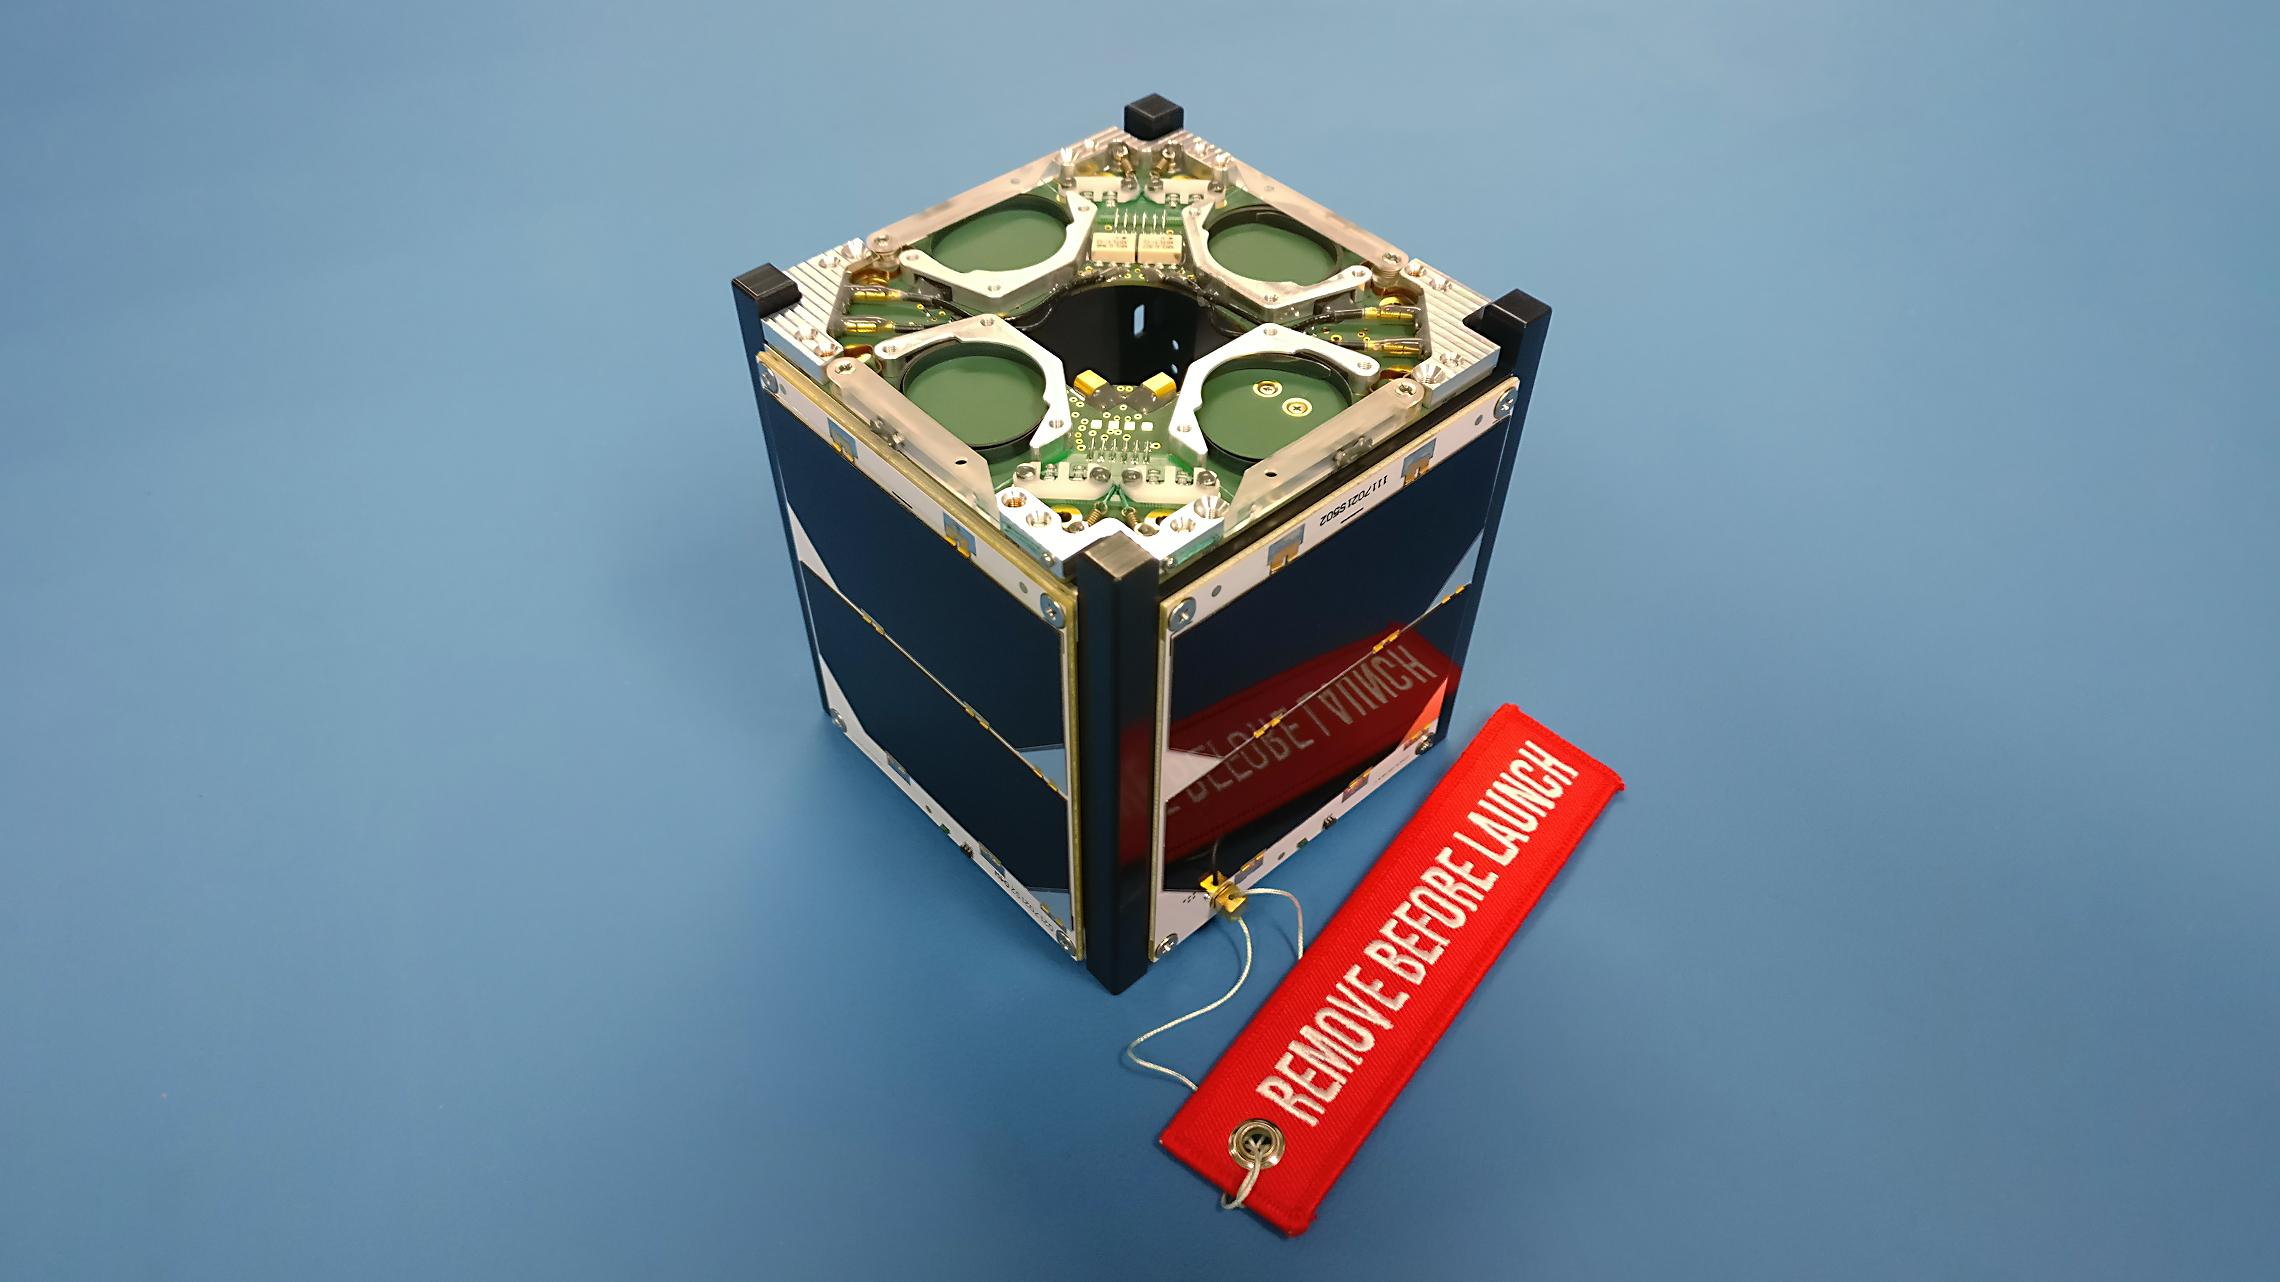
\includegraphics[width=\linewidth]{images/istsat1.jpeg}
		\caption{A caption.}
    \end{subfigure}
	\hspace{0.05\textwidth}
    \begin{subfigure}[t]{0.3\textwidth}
        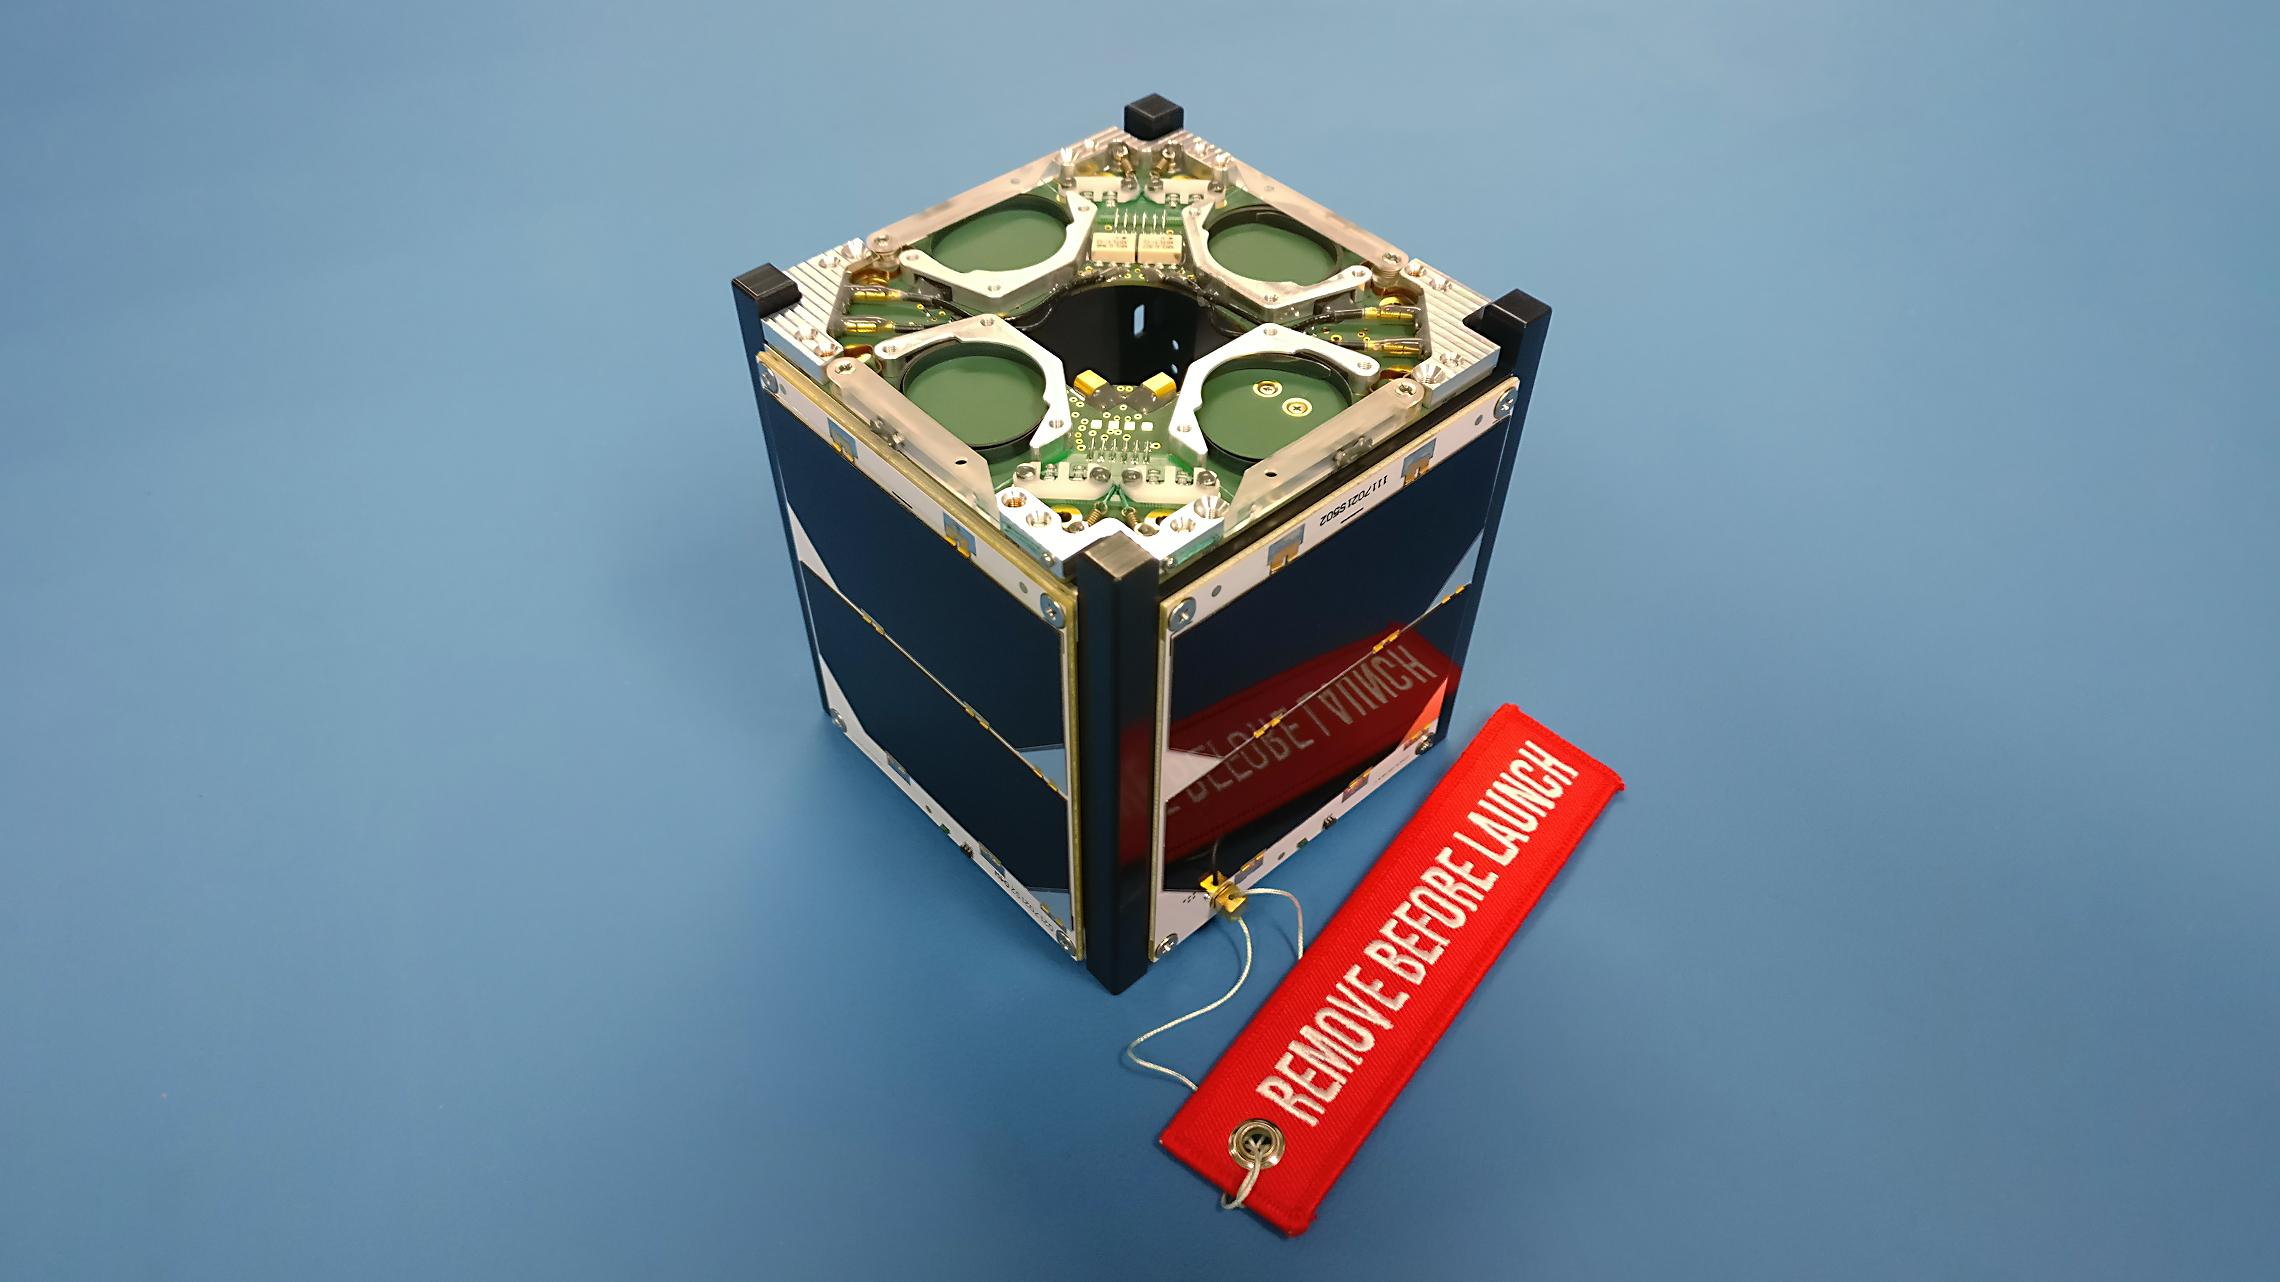
\includegraphics[width=\linewidth]{images/istsat1.jpeg}
		\caption{A caption.}
    \end{subfigure}

    \caption{This example is using the subfigure environment.}
	\label{fig:five_images}
\end{figure}

\chapter{Conclusions}
\label{chapter:conclusions}

To sum up, \LaTeX is not hard, it's just a bit annoying! However, having a cool template to start from and several useful code snippets will definitely make your life a bit easier. Anyways, here's a photo of my dog at the beach to help you get started with your writing:

\begin{figure}[!htb]
	\centering
	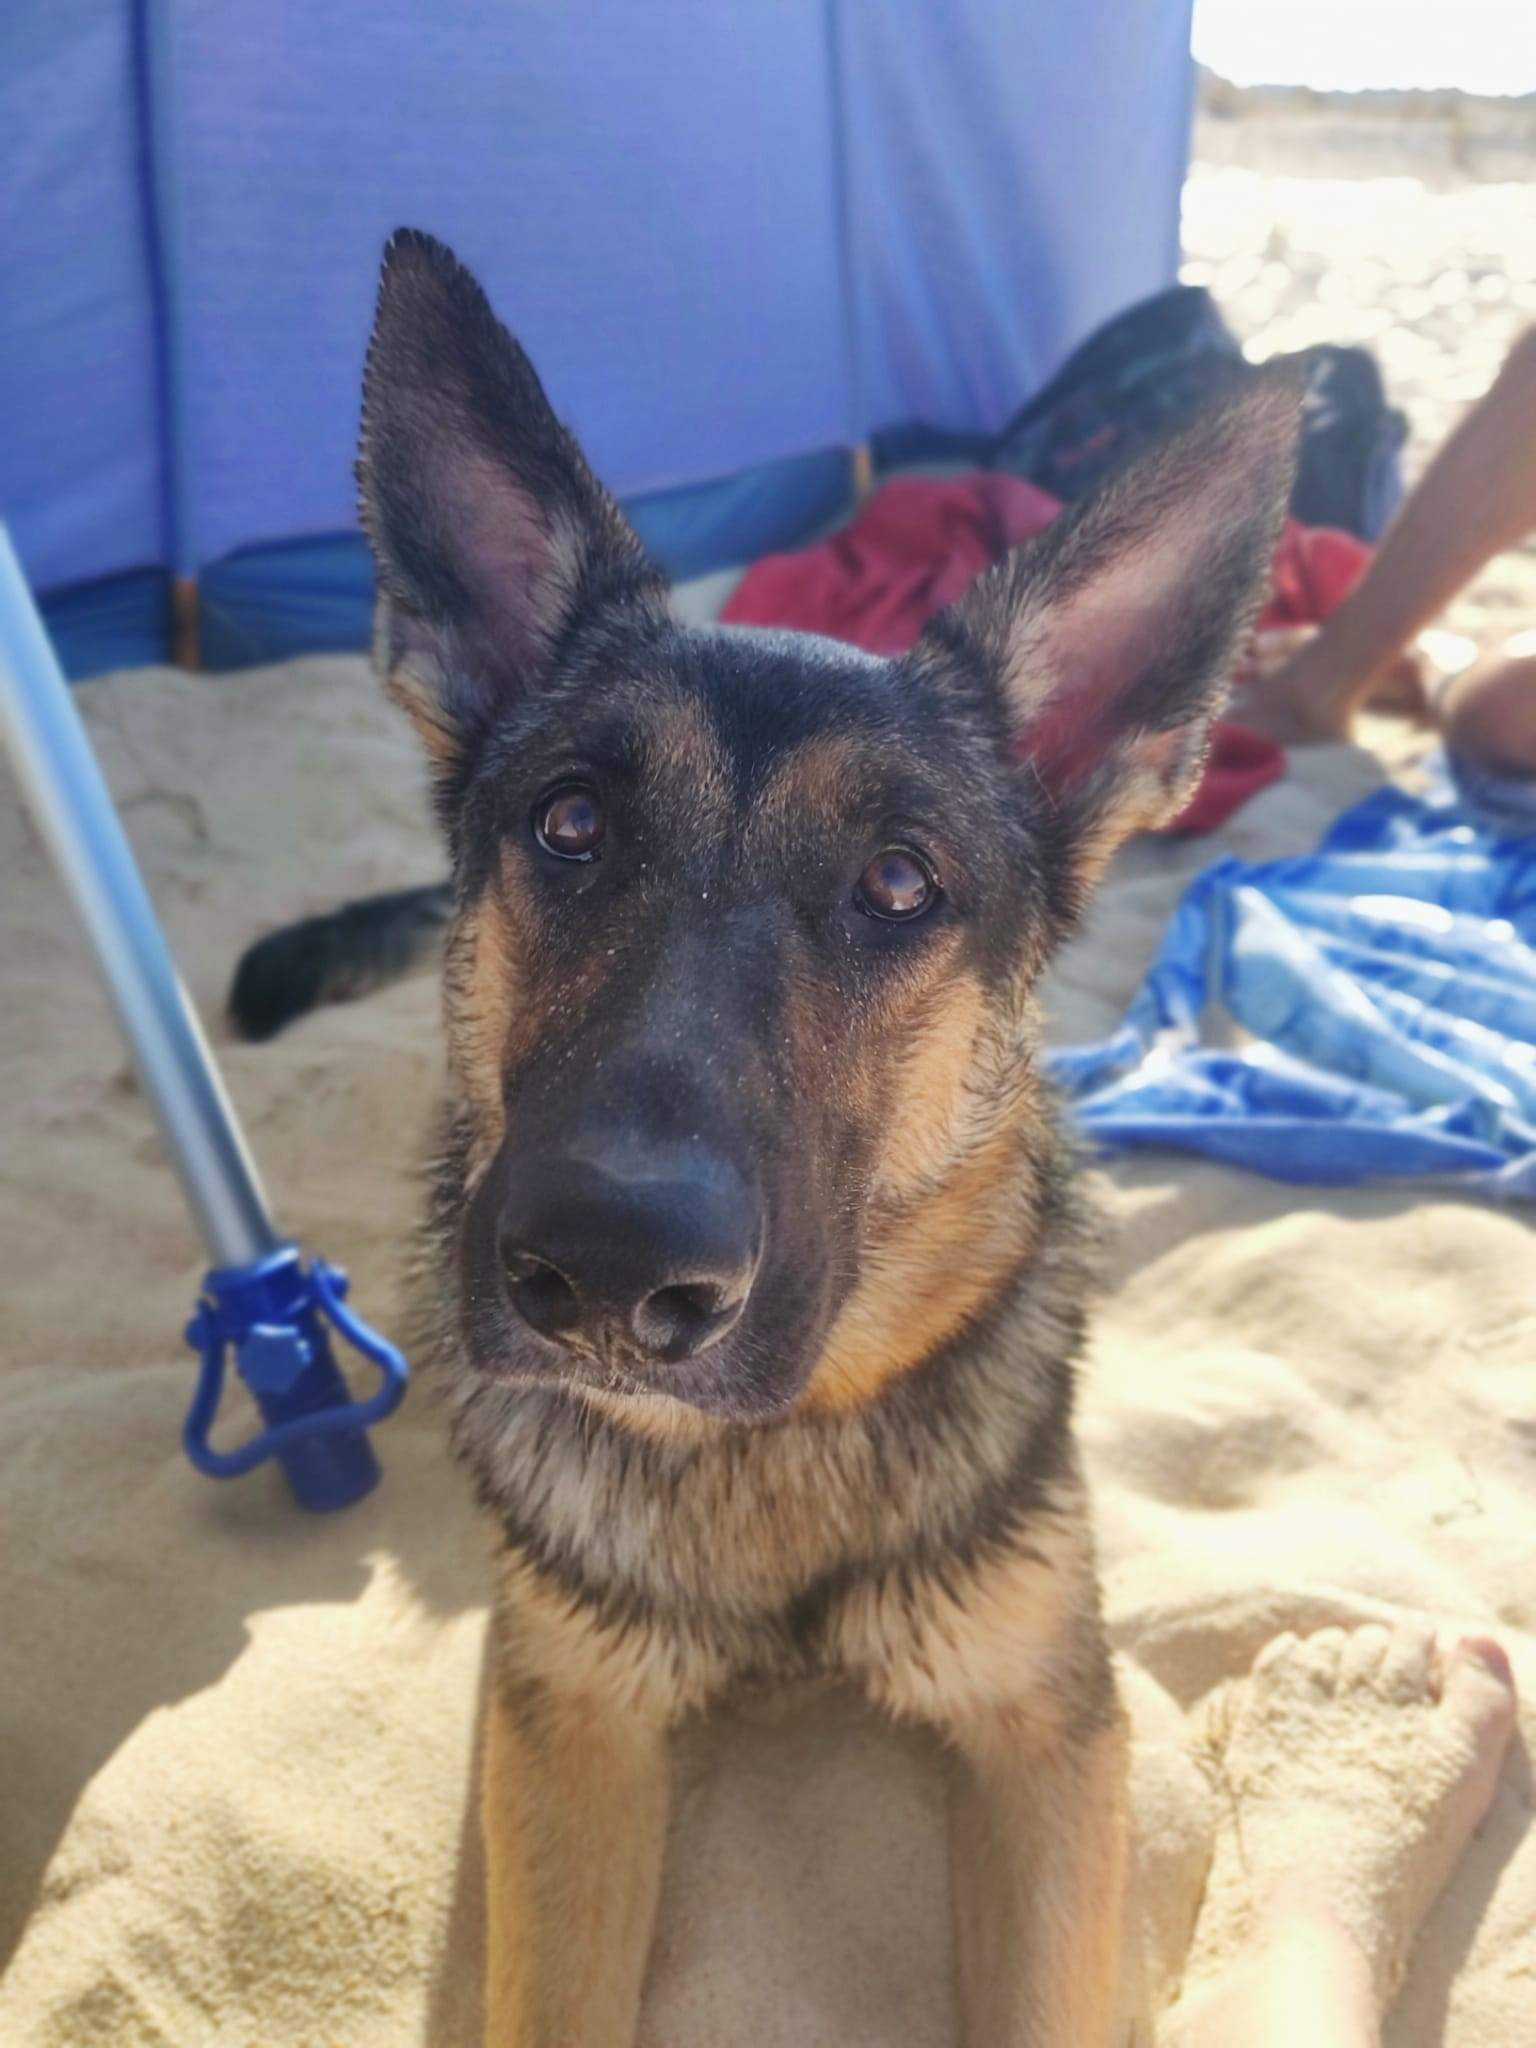
\includegraphics[width=.3\textwidth]{images/lira.jpeg}
	\caption{The goodest girl at the beach.}
\end{figure}

Hope this template helped you!


% ----------------------------------------------------------------------
%  Bibliography
% ----------------------------------------------------------------------
\phantomsection
\addcontentsline{toc}{chapter}{\bibname}
\bibliography{references}

% ----------------------------------------------------------------------
%  Attachments
% ----------------------------------------------------------------------
\appendix

\chapter{An important appendix}

You can include whatever in the appendices section. This may include other documents, images or code. Here is an image of Gasparzinho! You can learn more about Gasparzinho on \href{https://110.tecnico.ulisboa.pt/arquivos/episodio-58-gasparzinho/}{this} podcast.

\begin{figure}[!htb]
	\centering
	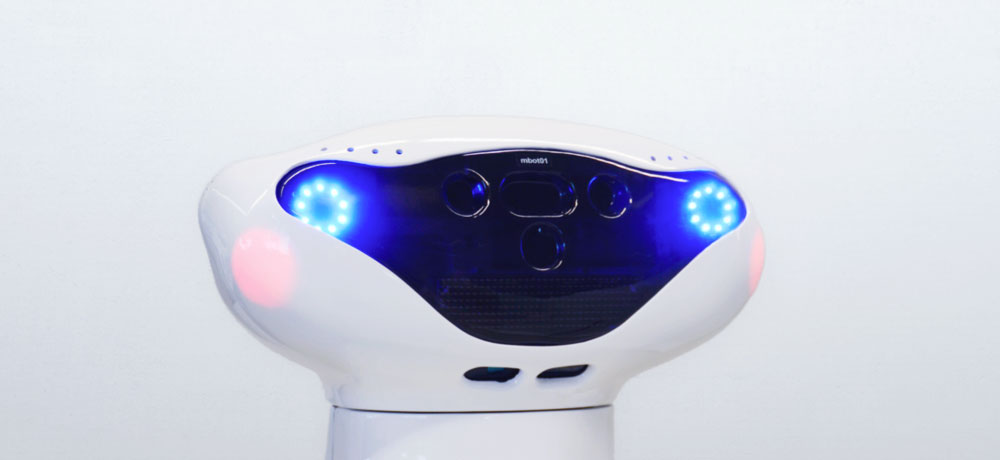
\includegraphics[width=.8\textwidth]{images/monarch.jpg}
\end{figure}

\end{document}